% !TeX root = er.tex

\chapter{Mouvement robotique et odométrie}\label{ch.motion}

Les algorithmes robotiques des chapitres précédents réagissent aux données provenant de leurs capteurs en modifiant la vitesse et la direction de leur mouvement, mais ces modifications ne sont pas quantitatives. Nous n'avons pas demandé aux robots de se déplacer deux fois plus vite ou de tourner $90^\circ$ vers la droite. Dans le monde réel, les robots doivent se déplacer vers des endroits spécifiques et peuvent avoir des contraintes techniques sur la vitesse de leur déplacement ou sur leur rotation. Ce chapitre présente les mathématiques du mouvement robotique.

Les sections~\ref{s.distance-vitesse}--\ref{s.acceleration} passent en revue les concepts de distance, de temps, de vitesse et d'accélération qui devraient être familiers lors de l'introduction à la physique. La physique du mouvement leur généralement enseignée à l'aide du calcul, mais un ordinateur ne peut pas traiter des fonctions continues ; il faut donc utiliser des approximations discrètes, comme décrit dans la section~\ref{s.continuous}.

Les sections~\ref{s.odometry}--\ref{s.odometry-turns} présentent la \emph{l'odométrie}, l'algorithme fondamental pour le calcul du mouvement robotique. Une approximation de la position d'un robot peut être obtenue en calculant de manière répétée la distance parcourue et le changement de direction à partir de la vitesse des roues dans un court laps de temps. Malheureusement, l'odométrie est sujette à de graves erreurs, comme le montre la section~\ref{s.odometry-errors}. Il est important à noter que les erreurs de direction sont beaucoup plus importantes que les erreurs de distance.

Dans l'implémentation la plus simple, la vitesse des roues d'un robot est supposée être proportionnelle à la puissance appliquée par les moteurs. La section~\ref{s.wheel} montre comment la précision de l'odométrie peut être améliorée en utilisant des \emph{codeurs de roue}, qui mesurent le nombre réel de tours des roues.

La section~\{ref{s.imu} présente une vue d'ensemble de la \emph{navigation inertielle}, qui est une forme sophistiquée d'odométrie basée sur la mesure de l'accélération linéaire et angulaire, puis sur l'intégration pour obtenir la vitesse et la position. Les capteurs de navigation inertielle (accéléromètres et gyroscopes) étaient autrefois très coûteux, ce qui limitait son application aux avions et aux fusées, mais une nouvelle technologie appelée \emph{systèmes micro-électromécaniques} a permis de construire des robots dotés de la navigation inertielle.

Les voitures ne peuvent pas se déplacer de haut en bas, contrairement aux hélicoptères et aux sous-marins qui ont une plus grande liberté de mouvement. Cela s'exprime par le concept de \emph{degrés de liberté (DOF)} qui fait l'objet de la section~\ref{s.dof}. La section~\ref{s.num-actuators} traite de la relation entre les DOF et le nombre \emph{d'actuateurs} (moteurs) dans un système robotique.

Le nombre de DOF d'un système ne signifie pas que le système, par exemple un véhicule, peut se déplacer librement dans toutes ces directions. Une voiture peut se déplacer en tout point du plan et s'orienter dans n'importe quelle direction, mais elle ne peut pas se déplacer latéralement, ce qui nécessite une manœuvre difficile lors d'un stationnement parallèle. Cela est dû à la différence entre les DOF et les \emph{degrés de mobilité (DOM)}, un sujet exploré dans la section~\ref{s.holonomic}, ainsi que le concept de \emph{mouvement holonome} qui relie les DOF et les DOM.

\section{Distance, vitesse et temps}\label{s.distance-vitesse}

Supposons qu'un robot se déplace avec une \emph{vitesse}\index{vitesse} constante de $10$ cm/s pendant une période de \emph{temps} de $5$ s.\footnote{La vitesse est une \emph{vitesse} dans une \emph{direction}. Un robot peut se déplacer de $10$ cm/s en avant ou en arrière ; dans les deux cas, la vitesse est la même mais la vélocité est différente.} La \emph{distance} qu'il parcourt est de $50$ cm. En général, si un robot se déplace à une vitesse constante de $v$ pendant une période de temps de $t$, la distance qu'il parcourt est de $s=vt$. Lorsque les moteurs sont alimentés, les roues tournent, ce qui entraîne le déplacement du robot à une certaine vitesse. Cependant, nous ne pouvons pas spécifier qu'une certaine puissance entraîne une certaine vitesse :

\begin{itemize}
\item Deux composants électriques ou mécaniques ne sont jamais exactement identiques. Un moteur est composé d'aimants et de câbles électriques dont l'interaction entraîne la rotation d'un arbre mécanique. De petites différences dans les propriétés de l'aimant et du fil, ainsi que de petites différences dans la taille et le poids de l'arbre, peuvent faire que les arbres de deux moteurs tournent à des vitesses légèrement différentes pour la même puissance.

\L'environnement affecte la vitesse d'un robot. Une friction trop faible (glace) ou trop forte (boue) peut ralentir le déplacement d'un robot par rapport à une surface pavée sèche.

\item Les forces externes peuvent affecter la vitesse d'un robot. Il a besoin de plus de puissance pour maintenir une vitesse spécifique lorsqu'il se déplace en montée et de moins de puissance lorsqu'il se déplace en descente, car la force de gravité diminue et augmente la vitesse. Faire du vélo à une vitesse constante face au vent demande plus d'effort que de rouler avec le vent, et un vent latéral rend la relation entre la puissance et la vitesse encore plus compliquée.
\end{itemize}

Puisque $s=vt$, il suffit de mesurer deux de ces quantités pour calculer la troisième. Si nous mesurons la distance et le temps, nous pouvons calculer la vitesse comme $v=s/t$. Les distances relativement courtes (jusqu'à plusieurs mètres) peuvent être mesurées avec précision (à 1 cm près) à l'aide d'une règle ou d'un mètre ruban. L'application chronomètre d'un smartphone peut mesurer le temps avec précision (centièmes de seconde).

\begin{framed}
\act{Vélocité sur une distance fixe}{velocity}
\begin{itemize}
\item Écrivez un programme qui règle votre robot sur une puissance avant constante.
\item Marquez deux lignes distantes de $1$ m sur le sol. Utilisez un chronomètre pour mesurer le temps que met le robot à se déplacer entre les lignes. Calculez la vitesse du robot. Exécutez le programme dix fois et enregistrez les vitesses. Les vitesses varient-elles ?
\item Placez le robot sur le sol et faites-le fonctionner pendant $5$ s. Mesurez la distance qu'il parcourt. Calculez sa vitesse. Exécutez le programme dix fois et enregistrez les vitesses. Les vitesses varient-elles ?
\item Quelle méthode donne des résultats plus précis ?
\item Répétez cette expérience sur différentes surfaces et discutez des résultats.
\end{itemize}
\end{framed}

L'activité~\ref{act.velocity} montre que pour un réglage de puissance constant, la vitesse d'un robot peut varier de manière significative. Pour naviguer avec précision dans un environnement, un robot doit détecter les objets de son environnement, tels que les murs, les marques au sol et les objets.

\section{Accélération en tant que changement de vitesse}\label{s.acceleration}

L'activité~\ref{act.velocity} a spécifié des paramètres de puissance constante et la vitesse du robot sera donc (plus ou moins) constante. Que se passe-t-il lorsque la vitesse varie ?


\begin{framed}
\act{Changement de vitesse}{change-v}
\begin{itemize}
\item Exécutez le premier programme de l'activité~\ref{act.velocity} en faisant varier la distance entre les marques : $0,25$ m, $0,5$ m, $1$ m, $1,5$ m, $2$ m. Pour chaque distance, exécutez le programme plusieurs fois et prenez la moyenne des vitesses calculées. Les vitesses sont-elles les mêmes pour chaque distance ?
\item Pour améliorer la précision de la mesure, placez des marques sur le sol à ces distances et utilisez le minuteur du robot pour enregistrer les moments où les marques sont détectées.
\end{itemize}
\end{framed}

Dans l'activité~\ref{act.change-v}, vous constaterez que pour les distances les plus longues, les vitesses seront proches les unes des autres, mais que pour les distances plus courtes, les vitesses seront considérablement différentes. La raison en est que la formule $v=s/t$ suppose que la vitesse est constante sur toute la distance. En réalité, un véhicule doit changer sa vitesse pour passer de l'arrêt à une vitesse constante. De même, un véhicule doit décélérer pour s'arrêter.

Pour obtenir une image fidèle du mouvement d'un robot, nous devons diviser son mouvement en petits segments $s_1,s_2,\ldots$ :
\begin{center}
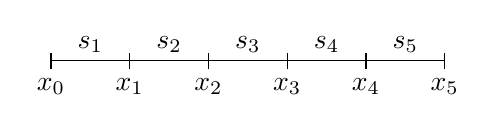
\begin{tikzpicture}
\draw (0,0) -- (5,0) ;
\foreach \x/\l in {.5cm/$s_1$, 1.5cm/$s_2$, 2.5cm/$s_3$, 3.5cm/$s_4$, 4.5cm/$s_5$}
  \node at (\x,2mm) {\l} ;
\foreach \x/\l in {0cm/$x_0$, 1cm/$x_1$, 2cm/$x_2$, 3cm/$x_3$, 4cm/$x_4$, 5cm/$x_5$}
  \draw (\x,-1mm) -- (\x,1mm) node [below,yshift=-2mm] {\l} ;
\end{tikzpicture}
\end{center}
et mesurer la distance et le temps pour chaque segment individuellement. Ensuite, nous pouvons calculer les vitesses pour chacun de ces segments. Si nous désignons la longueur du segment $s_i$ par $\Delta s_i = x_{i+1}-x_i$ et le temps que met le robot à traverser le segment $s_i$ par $\Delta t_i = t_{i+1}-t_i$, alors $v_i$, la vitesse dans le segment $s_i$ est donnée par :
\[v_i = \frac{\Delta s_i}{\Delta t_i}\,.\]

La figure~\ref{fig.instant-v} est un graphique de la distance en fonction du temps pour un robot en accélération. L'axe du temps a été divisé en segments et les pentes $\displaystyle\frac{\Delta s_i}{\Delta t_i}$ montrent la vitesse moyenne dans chaque segment, qui augmente avec le temps.

\begin{figure}
\begin{center}
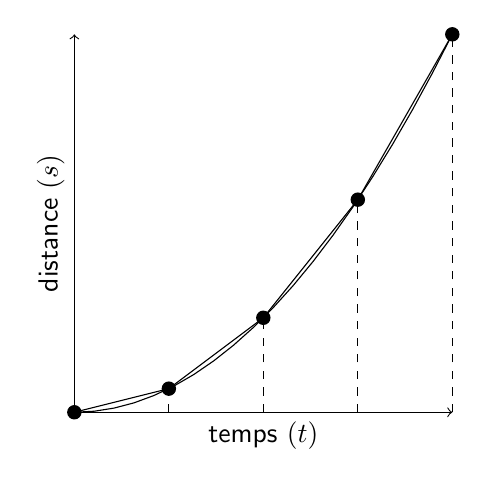
\begin{tikzpicture} [scale=1.2,samples=20,domain=0:4]
\draw[<->] (4,0) -- node [below] {\textsf{temps} ($t$)} (0,0) -- node [sloped,above] {\textsf{distance} ($s$)} (0,4) ;
\draw plot (\x,{\x*\x/4}) ;
\draw [mark=*] plot coordinates {(0,0) (1, .25) (2,1) (3,2.25) (4,4)} ;
\draw[dashed] (1,0) -- (1,.25) ;
\draw[dashed] (2,0) -- (2,1) ;
\draw[dashed] (3,0) -- (3,2.25) ;
\draw[dashed] (4,0) -- (4,4) ;
\end{tikzpicture}
\caption{Un robot en accélération : la distance augmente au carré du temps}\label{fig.instant-v}
\end{center}
\end{figure}

\emph{L'accélération} est définie comme la variation de la vitesse sur une période de temps :
\[a_i = \frac{\Delta v_i}{\Delta t_i}\,.\]
Lorsque la puissance du robot est réglée sur une valeur fixe, la force appliquée au robot est constante et nous nous attendons à ce que l'accélération reste constante, ce qui augmente la vitesse. Cependant, à un certain point, l'accélération est réduite à zéro, ce qui signifie que la vitesse n'augmente plus, car la puissance appliquée aux roues est juste suffisante pour surmonter le frottement de la route et la résistance du vent.

Voyons ce qui se passe si l'on augmente la puissance avec le temps.

\begin{framed}
\act{Accélération}{accel}
\begin{itemize}
\item Écrivez un programme qui fait accélérer le robot en augmentant périodiquement la puissance. Par exemple, démarrez le robot à une puissance de $20$ et augmentez-la à $40$ après $1$ s, puis à $60$ après $2$ s, à $80$ après $3$ s, et enfin à $100$ après $4$ s.
\item Placez le robot sur la piste et exécutez le programme.
\item Enregistrez les distances entre chaque changement de réglage de la puissance. Calculez et tracez les vitesses dans chacun de ces segments.
\end{itemize}
\end{framed}


\section{Des segments au mouvement continu}\label{s.continuous}

Au fur et à mesure que la taille des segments diminue, nous obtenons la vitesse instantanée\index{vitesse!instantanée} du robot en un seul point du temps, exprimée sous forme de dérivée :
\[v(t) = \frac{ds(t)}{dt}\,.\]
De la même manière, l'accélération instantanée du robot est définie comme suit :
\[a(t) = \frac{dv(t)}{dt}\,.\]
Pour une accélération constante, la vitesse peut être obtenue en intégrant la dérivée :
\[v(t) = \int a\, dt = a\int {dt} = at\,,\]
et ensuite la distance peut être obtenue en intégrant à nouveau :
\[s(t) = \int v(t) dt=\int a\,t\,dt = \frac{at^2}{2}\,.\]

\noindent{}\textbf{Exemple} Une voiture moyenne accélère de $0$ à $100$ km/h en environ $10$ s. Tout d'abord, nous convertissons les unités km/h en m/s :
\[
v_{\textit{max}} = 100\, \textrm{km/h} = \frac{100\cdot 1000}{60\cdot 60} \,\textrm{m/s} = 27,8 \,\textrm{m/s}\,.
\]
En supposant une accélération constante, $v_{\textrm{max}} = 27,8 = at = 10a$, l'accélération est donc de $2,78$ m/s$^{2}$ ($2,78$ mètres par seconde par seconde, c'est-à-dire que chaque seconde la vitesse augmente de $2,78$ mètres par seconde). La distance parcourue par la voiture en $10$ s est :
\[s(10) = \frac{at^2}{2} = \frac{2.78\cdot 10^2}{2}= 139 \,\textrm{m}\,.\]

\begin{framed}
\act{Computer la distance en accélérant}{distance-a}
\begin{itemize}
\item Pour différents véhicules (voitures de course, motos), recherchez le temps nécessaire pour accélérer de $0$ à $100$ km/h. Calculez la distance parcourue.
\item Supposez que l'accélération d'un véhicule augmente linéairement, c'est-à-dire que $a=kt$ pour une constante $k$. Que valent $v(t)$ et $s(t)$.
\item Pour plusieurs valeurs de $k$ et $t$, calculez les vitesses et distances finales.
\end{itemize}
\end{framed}

\begin{framed}
\act{Mesure du mouvement à accélération constante}{constant-a}
\begin{itemize}
\item Écrire un programme qui applique le réglage de la puissance maximale à un robot.
\item Placez le robot sur une surface et exécutez le programme.
\item Lorsque le robot semble avoir atteint sa vitesse maximale, enregistrez le temps écoulé depuis le début de l'exécution.
\item Comparez la distance mesurée à $s = at^2/2$ (Fig.~\ref{fig.acc-distance}).
\item Courez à nouveau et mesurez les distances à intervalles de temps fixes. Calculez les vitesses à partir des distances divisées par le temps et comparez-les à $v=at$ (Fig.~\ref{fig.acc-velocity}).
\item Dans certains robots, vous pouvez définir une vitesse cible et lire la vitesse réelle. Si votre robot peut le faire, comparez les vitesses mesurées avec les vitesses calculées.
\end{itemize}
\end{framed}

\begin{figure}
\begin{minipage}{.45\textwidth}
\begin{tikzpicture}[samples=20,domain=0:4]
\draw[<->] (4,0) -- node[below] {\textsf{temps} ($t$)} (0,0) -- node[sloped,above] {\textsf{vitesse} ($v$)} (0,4) ;
\draw plot (\x,{.5*\x}) ;
\end{tikzpicture}
\caption{Vélocité pour une accélération constante}\label{fig.acc-velocity}
\end{minipage}
\hspace{\fill}
\begin{minipage}{.45\textwidth}
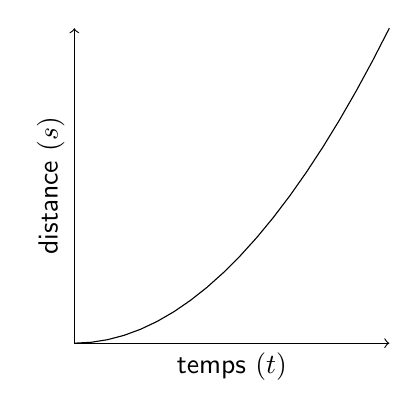
\begin{tikzpicture}[samples=20,domain=0:4]
\draw[<->] (4,0) -- node[below] {\textsf{temps} ($t$)} (0,0) -- node[sloped,above] {\textsf{distance} ($s$)} (0,4) ;
\draw plot (\x,{.5*\x*\x/2}) ;
\end{tikzpicture}
\caption{Distance pour une accélération constante}\label{fig.acc-distance}.
\end{minipage}
\end{figure}

\section{Navigation par odométrie}\label{s.odometry}
\index{odométrie}

Supposons que vous soyez dans une voiture et que votre système de navigation émette l'instruction suivante : "Dans 700 mètres, tournez à droite". Votre tâche est maintenant très simple : Observez l'odomètre de votre voiture qui mesure la distance que vous avez parcourue. Lorsque sa valeur approche des 700 mètres au-delà de sa valeur initiale, vous cherchez alors une rue à droite. L'odomètre d'une voiture mesure la vitesse et le temps, et multiplie ces deux valeurs pour calculer la distance parcourue.

\L'odométrie - la mesure de la distance - est une méthode fondamentale utilisée par les robots pour la navigation. La mesure du temps est facile grâce à l'horloge interne de l'ordinateur embarqué. La mesure de la vitesse est plus difficile : dans certains robots éducatifs, des encodeurs de roue sont utilisés pour compter les rotations des roues (section~\ref{s.wheel}), tandis que dans d'autres, la vitesse est estimée à partir des propriétés des moteurs. Connaissant la distance parcourue $s=vt$, la nouvelle position du robot peut être calculée. En une dimension, le calcul est trivial, mais il devient un peu plus complexe lorsque le mouvement implique des virages. Cette section présente le calcul de la distance par odométrie, d'abord pour un robot se déplaçant linéairement, puis pour un robot effectuant un virage.

La section~\ref{s.odometry-errors} montre que les erreurs de cap sont plus graves que les erreurs de distance.

L'un des inconvénients de l'odométrie (avec ou sans encodeurs de roue) est que les mesures sont indirectes : elles relient la puissance des moteurs ou le mouvement des roues aux changements de position du robot. Cela peut être source d'erreurs car la relation entre la vitesse du moteur et la rotation des roues peut être très non linéaire et varier dans le temps. En outre, les roues peuvent glisser et déraper, ce qui peut entraîner des erreurs dans la relation entre le mouvement des roues et le mouvement du robot. De meilleures estimations de la position peuvent être obtenues en utilisant un système de navigation inertiel, qui mesure directement l'accélération et la vitesse angulaire pouvant être utilisées pour déterminer la position du robot (section~\ref{s.imu}).

L'odométrie est une forme de \emph{localisation} : le robot doit déterminer sa position dans l'environnement. En odométrie, nous estimons la position en mesurant le changement par rapport à la position initiale connue du robot, tandis que la localisation proprement dite (Chap.~\ref{ch.local}) fait référence à la détermination de la position d'un robot par rapport aux positions connues d'autres objets tels que des points de repère ou des balises.

\section{Odométrie linéaire}
\index{odométrie!linéaire}

Avant d'étudier les mathématiques de l'odométrie, voyons l'activité suivante :

\begin{framed}
\act{Distance à partir de la vitesse et du temps}{odometry1}
\begin{itemize}
\item Faites bouger le robot à une puissance constante pendant une période donnée et mesurez la distance parcourue.
\item Répétez la mesure plusieurs fois. La distance est-elle constante ? Si non, de combien varie-t-elle en pourcentage de la distance ?
\item Répétez la mesure plusieurs fois pour différents réglages de puissance. La distance mesurée est-elle linéaire en fonction du réglage de la puissance ? La variation de la distance mesurée sur plusieurs parcours dépend-elle du réglage de la puissance ?
\item Répétez la mesure pour un réglage de puissance fixe mais pendant des périodes de temps différentes et analysez les résultats.
\end{itemize}
\end{framed}

Lorsqu'une relation entre la puissance du moteur et la vitesse $v$ a été déterminée, le robot peut calculer la distance parcourue par $s=vt$. S'il démarre à la position $(0,0)$ et se déplace en ligne droite le long de l'axe $x$, alors après $t$ secondes, sa nouvelle position est $(vt,0)$.

Cette activité doit démontrer qu'il est possible de mesurer une distance par odométrie avec une précision et une exactitude raisonnables. Une voiture autonome peut utiliser l'odométrie pour déterminer sa position afin de ne pas avoir à analyser continuellement les données de ses capteurs pour vérifier si la rue cherchée a été atteinte. Compte tenu des incertitudes du mouvement et de la route, la voiture ne doit pas dépendre uniquement de l'odométrie pour décider quand tourner, cependent l'erreur ne sera pas énorme et les données des capteurs peuvent être analysées pour détecter le virage lorsque l'odométrie indique que la voiture est à proximité de l'intersection.

L'activité~\ref{act.odometry1} demande de mesurer la distance parcourue dans une dimension. Trois informations doivent être calculées si le mouvement est en deux dimensions : la \emph{position} $(x,y)$ du robot par rapport à une origine fixe et son \emph{cap} $\theta$, la direction dans laquelle le robot pointe (Fig.~\ref{fig.pos-head}). Le triplet $(x,y,\theta)$ est appelé la \emph{pose}\index{pose} du robot. Si le robot commence à l'origine $(0,0)$ et se déplace en ligne droite selon un angle $\theta$ avec une vitesse $v$ pendant un temps $t$, la distance parcourue est $s=vt$. Sa nouvelle position $(x,y)$ est :
\begin{eqnarray*}
x &=& vt \cos \theta\\
y &=& vt \sin \theta\,.
\end{eqnarray*}

\begin{figure}
\begin{center}
\begin{tikzpicture} [scale=1.2]
\draw (-1,0) -- (4,0) ;
\draw (0,-1) -- (0,3) ;
\node at (-5mm,-4mm) { $(0,0)$ } ;
\pic[rotate=30,scale=.6] at (0,0) { robot } ;
\pic[rotate=30,scale=.6] at (30:3) { robot } ;
\draw[dashed] (30:3) -| (0,0) ;
\draw[dashed] (30:3) |- (0,0) ;
\node at (1.2,1.7) {$x$} ;
\node at (2.8,.5) {$y$} ;
\draw[->] (30:3) -- +(30:1.2) {} ;
\draw[->] (0,0) -- +(30:1.2) {} ;
\node at (1,.3) {$\theta$} ;
\end{tikzpicture}
\caption{Position et cap}\label{fig.pos-head}
\end{center}
\end{figure}


\section{Odométrie avec virages}\label{s.odometry-turns}
\index{odométrie!tours@avec tours}

Supposons que le robot tourne légèrement à gauche car la roue droite se déplace plus rapidement que la roue gauche (Fig.\ref{fig.small-turn}). Sur la figure, le robot est orienté vers le haut de la page ; le point bleu représente la roue gauche, le point rouge la roue droite et le point noir le centre du robot qui se trouve à mi-chemin entre les roues. La \textit{ligne de base} $b$ est la distance entre les roues, et $d_l, d_r, d_c$ représentent les distances parcourues par les deux roues et le centre lorsque le robot tourne. Nous voulons calculer la nouvelle position et le nouveau cap du robot.

Nous pouvons mesurer $d_l$ et $d_r$, les distances parcourues par les deux roues en utilisant la méthode décrite dans l'activité~\ref{act.odometry1} : relier la puissance du moteur à la vitesse de rotation, puis multiplier par le temps. On peut aussi utiliser le nombre de rotations comptées par les encodeurs des roues. Si le rayon d'une roue est de $R$ et que les vitesses de rotation des roues gauche et droite sont respectivement de $\omega_l,\omega_r$ tours par seconde, alors après $t$ secondes la roue s'est déplacée :
\begin{equation}
d_i=2\pi R \omega_i t,\;\;\;i=l,r\,. \label{eq.rotation}
\end{equation}
La tâche consiste à déterminer la nouvelle pose du robot après le déplacement des roues sur cette distance.

\begin{figure}
\begin{center}
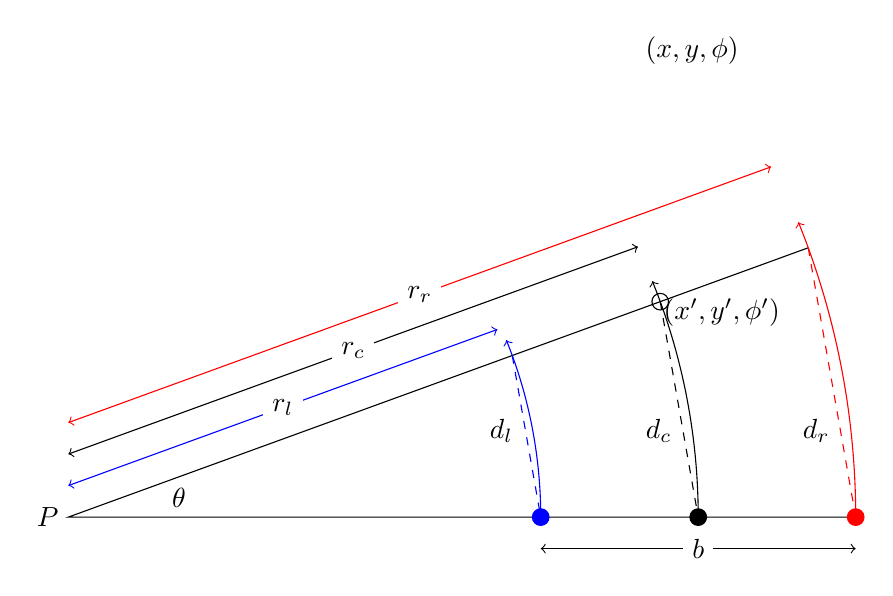
\begin{tikzpicture}
% Tracez des lignes d'angle
\draw (10,0) -- %
  (0,0) coordinate(origin) node [right=40pt,above] {$\theta$} -- %
  (20:10) ;
\node [left] at (0,0) {$P$} ;
% Flèches avec ligne de base
\draw[<->] (6,-.4) -- %
  node[fill=white] {$b$} (10,-.4) ;
% Trois : gros points, arcs, lignes pointillées, étiquettes
\foreach \x/\d/\c in {6/$d_l$/blue,8/$d_c$/black,10/$d_r$/red}
{
  \draw[dashed,\c] (20:\x) -- (\x,0) ;
  \draw[->,\c] (\x,0) arc (0:22:\x) ;
  \node at (\x-.5,1.1) {\d} ;
  \draw[fill,\c] (\x,0) circle [radius=3pt] ;
}
\draw[<->,blue] (0,4mm) -- node [black,fill=white] {$r_l$} +(20:58mm) ;
\draw[<->,black] (0,8mm) -- node[black,fill=white] {$r_c$} +(20:77mm) ;
\draw[<->,red] (0,12mm) -- node [black,fill=white] {$r_r$} +(20:95mm) ;
\node at (8,6, .2) {$(x,y,\phi)$} ;
\node at (8.3,2.6) {$(x',y',\phi')$} ;
\draw (20:8) circle [radius=3pt] ;
\end{tikzpicture}
\end{center}
\caption{Géométrie d'un virage à gauche par un robot à deux roues}\label{fig.small-turn}
\end{figure}

La figure~\ref{fig.small-turn} montre le robot initialement à la pose $(x,y,\phi)$, où le robot est orienté vers le nord ($\phi=\pi/2$). Après une rotation de $\theta$ radians, quelle est la nouvelle position $(x',y',\phi')$ ? Il est clair que le cap du robot est maintenant $\phi'=\phi+\theta$, mais nous devons également calculer $x',y'$.

La longueur d'un arc d'angle $\theta$ radians est donnée par sa fraction de la circonférence du cercle : $2\pi r\,(\theta/2\pi)=\theta r$. Pour les petits angles, les distances $d_l,d_c,d_r$ sont approximativement égales à la longueur des arcs correspondants, on a donc :
\begin{eqnarray}
\theta &=& d_l/r_l = d_c/r_c = d_r/r_r\,,\label{eqn.theta}
\end{eqnarray}
où $r_l$, $r_r$, $r_c$ sont les distances par rapport à $P$, l'origine du tour.

Les distances $d_l$ et $d_r$ sont obtenues à partir des rotations des roues (Eq.~\ref{eq.rotation}) et la ligne de base $b$ est une mesure physique fixe du robot. À partir de l'équation ~\ref{eqn.theta}, l'angle $\theta$ peut être calculé :
\begin{eqnarray*}
\theta r_r &=& d_r\\
\theta r_l &=& d_l\\
\theta r_r - \theta r_l &=& d_r - d_l\\\\
\theta &=& (d_r - d_l) / (r_r - r_l)\\\
\theta &=& (d_r - d_l) / b\,.
\end{eqnarray*}
Le centre est à mi-chemin entre les roues $r_c =(r_l+r_r)/2$,
donc encore une fois par l'équation suivante :
\begin{eqnarray*}
d_c&=&\theta r_c\\\\\
&=&\theta \left(\frac{r_l+r_r}{2}\right)\\
&=&\frac{\theta}{2} \left(\frac{d_l}{\theta} + \frac{d_r}{\theta}\right)\\\
&=&\frac{d_l+d_r}{2}\,.
\end{eqnarray*}

Si la distance parcourue est faible, la droite notée $d_c$ est approximativement
perpendiculaire au rayon passant par la position finale du robot. Par des triangles similaires, on voit que $\theta$ est la variation du cap du robot (Fig.~\ref{fig.heading}). Par trigonométrie :\footnote{Vous vous attendiez probablement à $\cos$ pour $dx$ et $\sin$ pour $dy$. Ce serait le cas si le robot était orienté selon l'axe $x$. Cependant, la position initiale est $\phi=\pi/2$ et nous avons $\sin(\theta+\pi/2)=\cos\theta$ et $\cos(\theta+\pi/2)=-\sin\theta$.}
\begin{eqnarray*}
\textit{dx} &=& - d_c \sin \theta\\\\
\textit{dy} &=& d_c \cos \theta\,,
\end{eqnarray*}
donc la pose du robot après le virage est :
\[
(x',y',\phi') = ( - d_c \sin \theta, d_c \cos \theta, \phi+\theta)\,.
\]

\begin{figure}
\begin{center}
\begin{tikzpicture}
% Draw angle with thetas
\draw (10,0) coordinate (A) -- %
  (0,0) coordinate (origin) node [right=40pt,above] {$\theta$} -- %
  (20:9) coordinate (B) node [xshift=1.5mm,yshift=-7mm] {$\theta$};
% Dashed line to complete the triangle
\draw[dashed] (A) -- node [right=1pt] {$d_c$} (B);
% Dashed perpendicular lines
\draw[dashed] (B) -- node [left] {$d_y$} ({B} |- {A}) coordinate (C);
\draw[dashed] (A) node[above left,xshift=1pt,yshift=14pt] {$\theta$} -- (A |- B);
% Dummy line for placing dx label
\path (C) -- node [below=1pt] {$d_x$} (A);
% Rectangles for right angles
\draw (C) rectangle +(6pt,6pt);
\draw[rotate=20] (B) rectangle +(-6pt,-6pt);
\end{tikzpicture}
\end{center}
\caption{Changement d'intitulé}\label{fig.heading}
\end{figure}

Les formules montrent comment calculer les changements \textit{dx}, \textit{dy} et $\theta$ lorsque le robot se déplace sur une courte distance. Pour calculer l'odométrie sur de plus longues distances, ce calcul doit être effectué fréquemment. Deux raisons expliquent pourquoi les intervalles entre les calculs doivent être courts : (a) l'hypothèse d'une vitesse constante ne vaut que pour les courtes distances et (b) le calcul trigonométrique est simplifié en supposant que la distance parcourue est courte.

\begin{framed}
\act{Odométrie en deux dimensions}{odométrie2}
\begin{itemize}
\item Écrivez un programme qui fait faire un léger virage à gauche au robot en temps donné.
\item Calculez la pose $( - d_c \sin \theta, d_c \cos \theta, \theta)$ et comparez le résultat avec les valeurs mesurées à l'aide d'une règle et d'un rapporteur. Exécutez le programme plusieurs fois et voyez si les mesures sont cohérentes.
\item Exécutez le programme pour différentes durées. Comment cela affecte-t-il l'exactitude et la précision du calcul de l'odométrie ?
\end{itemize}
\end{framed}

\section{Erreurs en odométrie}\label{s.odometry-errors}

Nous avons déjà noté que l'odométrie n'est pas précise car les mesures incohérentes et les irrégularités de la surface peuvent provoquer des erreurs. Dans cette section, nous montrons que même de petits changements dans la direction du mouvement du robot peuvent causer des erreurs beaucoup plus importantes que celles causées par des changements dans son mouvement linéaire.

Pour simplifier la présentation, supposons qu'un robot doive se déplacer de $10$ mètres depuis l'origine d'un système de coordonnées le long de l'axe $x$ et qu'il doive ensuite rechercher un objet spécifique dans son environnement. Quel est l'effet d'une erreur de $p\,\%$ ? Si l'erreur porte sur la mesure de $x$, la distance parcourue, alors $\Delta x$, l'erreur sur $x$ est :
\[\Delta x \leq \pm 10\cdot\frac{p}{100} = \pm\frac{p}{10}\ ; \textrm{meter}\,,\]
où la valeur est négative ou positive car le robot peut se déplacer jusqu'à $p\,\%$ avant ou après la distance prévue.

Supposons maintenant qu'il y ait une erreur de $p\%$ dans la \emph{direction} du robot et, pour simplifier, supposons qu'il n'y ait pas d'erreur dans la distance parcourue. La géométrie est la suivante :

\begin{center}
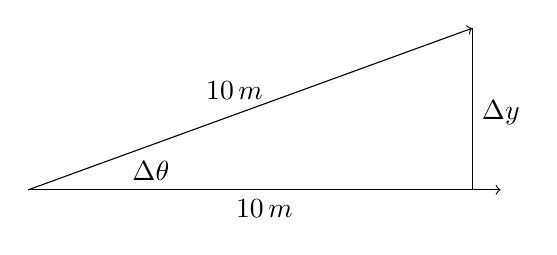
\begin{tikzpicture}
\draw[->] (0,0) -- node[below] {$10\,m$} (6,0);
\draw[->] (0,0) -- node[above,xshift=-2mm] {$10\,m$} +(20:6);
\draw (20:6) |- node[above right,yshift=7mm] {$\Delta y$} (0,0);
\node[above right,xshift=12mm] at (0,0) {$\Delta \theta$};
\end{tikzpicture}
\end{center}

Le robot avait l'intention de se déplacer de $10$ m le long de l'axe $x$, mais au lieu de cela, il s'est déplacé légèrement vers la gauche selon un angle de $\Delta \theta$. Calculons la déviation gauche-droite $\Delta y$. Par trigonométrie, $\Delta y = 10\sin \Delta\theta$. Une erreur de $p\,\%$ dans le cap est :
\[
\Delta\theta=360\cdot\frac{p}{100}=(3.6p)^\circ\,,
\]
donc la déviation gauche-droite est :
\[
\Delta y \leq \pm 10 \sin (3.6p)\,.
\]

Les tableaux suivants comparent la différence entre une erreur linéaire de $p\,\%$ (à gauche) et une erreur de cap de $p\,\%$ (à droite) :
\begin{displaymath}
\setlength{\arraycolsep}{2ex}
\renewcommand{\arraystretch}{1.1}
\begin{array}{r|r}
\multicolumn{1}{c|}{p\,\%} & \multicolumn{1}{c}{\Delta x \,(m)}\\\hline
1 & .1 \\
2 & .2 \\
5 & .5 \\
10 & 1.00\\
\end{array}
\;\;\;\;\;\;\;\;
\begin{array}{r|rrr}
\multicolumn{1}{c|}{p\,\%} & \multicolumn{1}{c}{\Delta \theta\,({}^\circ)} & \multicolumn{1}{c}{\sin\Delta\theta} & \multicolumn{1}{c}{\Delta y \,(\textrm{m})}\\\hline
1 & 3.6 & .063 & .63\\
2 & 7.2 & .125 & 1.25\\
5 & 18.0 & .309 & 3.09\\
10 & 36.0 & .588 & 5.88\\
\end{array}
\end{displaymath}

Pour une très petite erreur comme $2\,\%$, l'erreur de distance après un déplacement de $10$ m est de seulement $.2$ m, ce qui devrait placer le robot à proximité de l'objet qu'il recherche, mais une erreur de cap du même pourcentage place le robot à $1.25$ m de l'objet. Pour une erreur plus importante, telle que $5$ ou $10$, l'erreur de distance ($50$ ou $100$ cm) peut encore être gérée, mais l'erreur de cap place le robot à $3,09$ ou $5,88$ m, ce qui n'est même pas à proximité de l'objet.

L'accumulation des erreurs d'odométrie au fur et à mesure que la distance parcourue s'allonge est représentée sur la Fig.~\ref{fig.odo-errors}. La position initiale du robot est désignée par le point à l'origine.  En supposant une erreur d'au plus $\pm 4\,\%$ dans la direction linéaire et le cap, les positions possibles du robot après un déplacement de $d=1,2,\ldots,10$ mètres sont représentées par des ellipses. Les rayons mineurs des ellipses d'erreur résultent des erreurs linéaires :
\[.04s = 0.04, .08, \ldots, .4 \;\;\textrm{mètres},
\]
tandis que les rayons majeurs des ellipses d'erreur résultent des erreurs angulaires :
\[
d\sin \,(.04\cdot 360^\circ)=d \sin 14.4^\circ \approx{} .25, .50, \ldots 2.5\;\;\textrm{mètres}.
\]
Il est clair que les erreurs angulaires sont beaucoup plus importantes que les erreurs linéaires.

\begin{figure}
\begin{center}
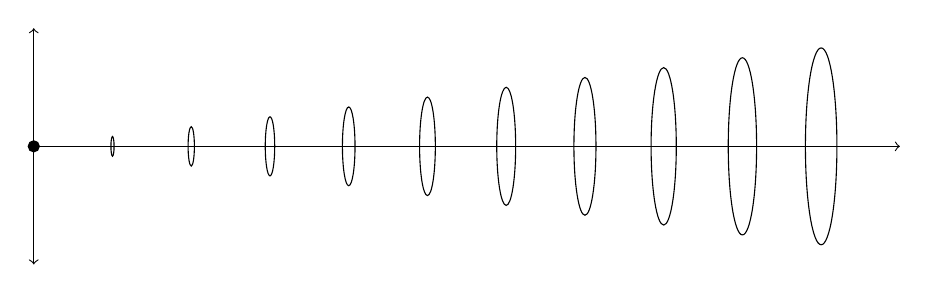
\begin{tikzpicture}
\draw[<->] (0,1.5) -- (0,-1.5);
\draw[->] (0,0) -- (11,0);
\draw[fill](0,0) circle[radius=2pt];
\foreach \x/\mult in {1/1, 2/2, 3/3, 4/4, 5/5, 6/6, 7/7, 8/8, 9/9, 10/10}
  \draw (\x,0) ellipse [x radius=\mult*.02cm, y radius=\mult*.125cm];
\end{tikzpicture}
\end{center}
\caption{Erreurs d'odométrie}\label{fig.odo-errors}
\end{figure}

Les erreurs étant inévitables, la position du robot calculée par odométrie doit être comparée périodiquement à une position absolue, qui devient la nouvelle position initiale pour les calculs ultérieurs. Les méthodes de détermination de la position absolue du robot sont présentées au Chap.~\ref{ch.local}.

\begin{framed}
\act{Ordres d'odométrie}{odo-error}
\begin{itemize}
\item Écrivez un programme pour que le robot se déplace en ligne droite sur $2$ mètres. Assurez-vous que la surface est lisse afin qu'il ne dévie pas de sa trajectoire et calibrez les paramètres du moteur afin que le robot se déplace aussi droit que possible.
\item Faites varier la puissance des moteurs des deux roues de façon à ce que le robot se déplace un peu plus lentement ou un peu plus rapidement qu'auparavant. Repérez sa position à intervalles fixes et voyez si l'erreur reste linéaire au cours du parcours.
\item Faites varier la puissance du moteur d'une roue de sorte que le robot tourne légèrement sur le côté. Repérez sa position à intervalles fixes et voyez si les erreurs sont proportionnelles au sinus de la différence entre le cap initial et le nouveau cap.
\end{itemize}
\end{framed}

\begin{framed}
\act{Effet combiné des erreurs d'odométrie}{odo-combine}
\begin{itemize}
\item Écrivez un programme qui fait en sorte que le robot se déplace en ligne droite sur $2$ mètres, puis tourne de $360^\circ$. Quelle est l'erreur de position du robot ?
\item Écrivez un programme qui fait tourner le robot de $360$, puis le fait se déplacer en ligne droite sur $2$ de distance. Quelle est l'erreur de position du robot ? Y a-t-il une différence entre cette erreur et celle de l'expérience précédente ?
\item Écrivez un programme qui permet au robot de se déplacer en ligne droite sur $2$ mètres, de faire un tour de $180^\circ$ et de se déplacer en ligne droite sur $2$ mètres. À quelle distance se trouve-t-il de sa position de départ ?
\end{itemize}
\end{framed}

\begin{framed}
\act{Correction des erreurs d'odométrie}{odo-correct}
\begin{itemize}
\item Modifiez le programme que vous avez écrit pour l'activité~\ref{act.odo-error} pour introduire \emph{jitter}, une variation aléatoire de la puissance fournie au moteur. Vérifiez que la distance parcourue par le robot en un temps donné n'est pas constante, mais varie légèrement d'une course à l'autre.
\item Marquez une ligne de but sur le sol et calculez le temps que le robot doit mettre pour atteindre le but.
\item Lorsque le robot s'est déplacé pendant ce laps de temps, voyez s'il peut trouver le but en avançant et en reculant par petits pas jusqu'à ce qu'il détecte le but.
\end{itemize}
\end{framed}

\section{Codeurs de roue}\label{s.wheel}
\index{Codeur de roue}

L'odométrie dans un véhicule à roues comme une voiture peut être améliorée en mesurant la rotation des roues au lieu de convertir la puissance du moteur en vitesse. La circonférence d'une roue est de $2\pi r$, où $r$ est le rayon de la roue en cm, donc si $n$ rotations sont comptées, nous savons que le robot s'est déplacé de $2\pi n r$ cm. Il est possible de construire des encodeurs de roue qui mesurent des fractions de tour. Si un signal est généré $8$ fois par tour, la distance parcourue est de $2\pi nr /8$ cm, $n$ étant maintenant le nombre de signaux comptés par l'ordinateur.

Il existe de nombreuses façons différentes de mettre en œuvre les codeurs de roue. Une conception populaire consiste à utiliser une source de lumière telle qu'une diode électroluminescente (LED), un capteur de lumière et un disque de codage fixé à l'axe de la roue (Fig.~\ref{fig.wheel}). Le disque est perforé de trous (Fig.~\ref{fig.encoding-disk}) de sorte que chaque fois qu'un trou est opposé à la source lumineuse, le capteur génère un signal.

\begin{figure}
\begin{minipage}{.5\textwidth}
\begin{tikzpicture}[scale=.7]
% Draw axle
\draw[thick,fill=gray!80] (0,-.18) rectangle (5,.18) node[right=4pt,yshift=10pt,text width=8mm] {\textsf{au moteur}};
% Draw disk
\draw[rounded corners,fill=gray!10] (3,-1.6) node[right=10pt,yshift=3pt] {\textsf{disque d'encodage}} rectangle +(.4,3.2);
% Draw wheel
\draw[rounded corners,thick,fill=gray!20] (0,-2) to [bend left=10] (0,2) node[xshift=3.5mm,yshift=3mm] {\textsf{roue}} -- (1,2) to [bend left=10](1,-2) -- cycle;
\begin{scope}[xshift=20mm,yshift=8mm]
% LED
\draw[red] (0,0) rectangle node[black,above=12pt] {\textsf{LED}} (.3,.6);
\draw[red,bend right=90] (.3,0) to (.3,.6);
% Sensor
\draw[blue] (2,0) rectangle node[black,above=12pt] {\textsf{capteur}} (2.3,.6);
\draw[blue,bend left=90] (2,0) to (2,.6);
\end{scope}
\draw[raxis] (-15mm,0) -- (64mm,0);
\end{tikzpicture}
\caption{Codeur à roue optique}\label{fig.wheel}
\end{minipage}
\hspace{\fill}
\begin{minipage}{.45\textwidth}
\begin{center}
\begin{tikzpicture}[scale=.5,baseline=-14mm]
\draw[fill=gray!20] (0,0) circle [radius=25mm];
\draw[fill=white] (0,0) circle [radius=5mm];
\foreach \x/\y/\theta in {
  0/18/0, 0/-18/0, 18/0/90, -18/0/90,
  12.5/12.5/-45, -12.5/12.5/45, 12.5/-12.5/-135, -12.5/-12.5/135
} {
  \node [draw,fill=white,shape=rectangle,inner sep=0pt,minimum width=3mm,minimum height=5mm,anchor=center,rotate=\theta] at (\x mm,\y mm) {};
}
\draw[raxis] (0,0) -- (10pt,0);
\draw[raxis] (0,0) -- (-10pt,0);
\draw[raxis] (0,0) -- (0,10pt);
\draw[raxis] (0,0) -- (0,-10pt);
\end{tikzpicture}
\end{center}
\caption{Disque d'encodage\label{fig.encoding-disk}}
\end{minipage}
\end{figure}

La prise en charge des encodeurs de roue dans les robots éducatifs varie :
\begin{itemize}
\item Si un robot n'a pas d'encodeurs de roue, il doit être calibré ;
\item Le robot peut avoir des encodeurs de roue qui sont utilisés en interne ;
\item Certains robots comme le \lego{} Mindstorms permettent à l'utilisateur de lire les encodeurs.
\end{itemize}
L'activité suivante propose une expérience permettant de mesurer la distance parcourue en comptant les tours d'une roue. Elle peut être réalisée même si votre robot ne possède pas d'encodeurs de roue ou s'ils ne sont pas accessibles.

\begin{framed}
\act{Codage de roue}{roue}
\begin{itemize}
\item Faites une marque au sommet d'une roue du robot à l'aide d'une craie ou en fixant un étroit morceau de ruban adhésif de couleur. Écrivez un programme qui oblige le robot à se déplacer en ligne droite pendant une durée déterminée. Exécutez le programme et prenez une vidéo du côté du robot à l'aide de la caméra de votre smartphone.
\item Visionnez la vidéo et déterminez le nombre de tours en comptant le nombre de fois où la marque se trouve en haut de la roue.
\item Mesurez le rayon de la roue et calculez la distance parcourue. Dans quelle mesure le résultat est-il proche de la distance réelle mesurée sur le sol ?
\item Répétez la mesure en utilisant $n=2$ puis $n=4$ marques équidistantes sur la roue. Déterminez le nombre de tours en comptant le nombre de fois où une marque se trouve en haut de la roue et divisez par $n$. Calculez la distance.
\end{itemize}
\end{framed}

\section{Systèmes de navigation inertielle}\label{s.imu}
\index{inertial navigation system}

Un \emph{système de navigation inertielle (INS)} mesure directement l'accélération linéaire et la vitesse angulaire et les utilise pour calculer la position d'un véhicule. Le terme \emph{unité de mesure inertielle (IMU)} est également utilisé, mais nous préférons le terme INS qui fait référence à l'ensemble du système. L'intégration de l'accélération depuis la pose initiale jusqu'à l'instant présent $\tau$ donne la vitesse actuelle :
\[
v=\int_0^\tau a(t) \,dt\,.
\]
De même, l'intégration de la vitesse angulaire donne le changement de cap :
\[
\theta = \int_0^\tau \omega(t) \, dt\,.
\]
Dans un SIN, nous ne disposons pas de fonctions continues à intégrer ; l'accélération et la vitesse angulaire sont échantillonnées et la sommation remplace l'intégration :
\[
v_n = \sum^{n}_{i=0} a_n \Delta t,\;\; \theta_n = \sum^{n}_{i=0} \omega_n \Delta t\,.
\]
Les INS sont sujets à des erreurs dues à des imprécisions dans la mesure elle-même ainsi qu'à des variations causées par des facteurs environnementaux tels que la température, et par l'usure de l'unité. La mesure inertielle est souvent combinée avec le GPS (\ref{s.gps}) pour mettre à jour la position avec un emplacement absolu.

Les systèmes de navigation inertielle pour robots sont construits avec des \emph{systèmes micro-électromécaniques (MEMS)}\index{systèmes microélectromécaniques}, qui utilisent des techniques de fabrication de circuits intégrés combinant des éléments mécaniques avec des composants électroniques qui s'interfacent avec l'ordinateur du robot.

\subsection{Accelerometers}\label{s.accelerometer}
\index{inertial navigation system!accelerometer}

Si vous avez déjà pris l'avion, vous avez ressenti une force qui vous a poussé vers votre siège en raison de l'accélération rapide de l'avion au décollage. À l'atterrissage, vous êtes repoussé de votre siège. Vous pouvez également en faire l'expérience dans une voiture qui accélère rapidement ou qui effectue un arrêt d'urgence. L'accélération est liée à la force par la deuxième loi de Newton $F=ma$, où $m$ est la masse. En mesurant la force exercée sur un objet, on mesure l'accélération.

Les figures~\ref{fig.acc-forward}--\ref{fig.acc-backward} montrent comment un accéléromètre peut être construit à partir d'un objet (appelé masse) relié à un ressort. Plus l'accélération est importante, plus la force exercée par la masse sur le ressort est grande, ce qui entraîne la compression du ressort. La direction dans laquelle la masse se déplace donne le signe de l'accélération : vers l'avant ou vers l'arrière. L'ampleur de la force est mesurée indirectement en mesurant la distance parcourue par la masse. Vous pouvez constater que les diagrammes correspondent à notre expérience : lorsqu'une voiture accélère, vous êtes repoussé sur le siège, mais lorsqu'elle décélère (freine), vous continuez à avancer.

\begin{figure}
\begin{minipage}{.45\textwidth}
\begin{tikzpicture}[scale=.9]
\draw[->] (-40mm,17mm) -- node[w,midway] {\p{l'avant du véhicule}} (-8mm,17mm);
\draw (2mm,14mm) -- (-52mm,14mm) -- (-52mm,6mm) -- (2mm,6mm) -- cycle;
\draw (-50mm,10mm) -- (-52mm,10mm);
\draw (-50mm,10mm) -- ++(1mm,2mm) -- ++(1mm,-4mm) -- ++(1mm,4mm)  -- ++(1mm,-4mm) -- ++(1mm,4mm)  -- ++(1mm,-4mm) -- ++(1mm,4mm)  -- ++(1mm,-4mm) -- ++(1mm,4mm)  -- ++(1mm,-2mm) -- (-36mm,10mm);
\draw[fill] (-36mm,10mm) circle[radius=3mm];
\draw (0mm,10mm) -- (2mm,10mm);
\draw (0mm,10mm) -- ++(-3mm,2mm) -- ++(-3mm,-4mm) -- ++(-3mm,4mm)  -- ++(-3mm,-4mm) -- ++(-3mm,4mm)  -- ++(-3mm,-4mm) -- ++(-3mm,4mm)  -- ++(-3mm,-4mm) -- ++(-3mm,4mm)  -- ++(-3mm,-2mm) -- (-36mm,10mm);
\end{tikzpicture}
\caption{Accélération vers l'avant}\label{fig.acc-forward}
\end{minipage}
\hspace{\fill}
\begin{minipage}{.45\textwidth}
\begin{tikzpicture}[rotate=180,scale=.9]
\draw[<-] (-40mm,3mm) -- node[w,midway] {\p{l'avant du véhicule}} (-8mm,3mm);
\draw (2mm,14mm) -- (-52mm,14mm) -- (-52mm,6mm) -- (2mm,6mm) -- cycle;
\draw (-50mm,10mm) -- (-52mm,10mm);
\draw (-50mm,10mm) -- ++(1mm,2mm) -- ++(1mm,-4mm) -- ++(1mm,4mm)  -- ++(1mm,-4mm) -- ++(1mm,4mm)  -- ++(1mm,-4mm) -- ++(1mm,4mm)  -- ++(1mm,-4mm) -- ++(1mm,4mm)  -- ++(1mm,-2mm) -- (-36mm,10mm);
\draw[fill] (-36mm,10mm) circle[radius=3mm];
\draw (0mm,10mm) -- (2mm,10mm);
\draw (0mm,10mm) -- ++(-3mm,2mm) -- ++(-3mm,-4mm) -- ++(-3mm,4mm)  -- ++(-3mm,-4mm) -- ++(-3mm,4mm)  -- ++(-3mm,-4mm) -- ++(-3mm,4mm)  -- ++(-3mm,-4mm) -- ++(-3mm,4mm)  -- ++(-3mm,-2mm) -- (-36mm,10mm);
\end{tikzpicture}
\caption{Décélération (freinage)}\label{fig.acc-backward}
\end{minipage}
\end{figure}

\subsection{Gyroscopes}
\index{système de navigation inertielle!gyroscope}

Un \emph{gyroscope} (``gyro'') utilise le principe de la force de Coriolis pour mesurer la vitesse angulaire. Ce concept est expliqué dans les manuels de physique et nous ne nous y attarderons pas ici. Il existe de nombreux types de gyroscopes :
\begin{itemize}
\item Les gyroscopes classiques possèdent des disques mécaniques en rotation qui sont montés sur des cardans de sorte que l'axe de rotation reste fixe dans l'espace. Ces gyroscopes sont extrêmement précis mais sont très lourds et consomment beaucoup d'énergie. On les trouve sur les véhicules de grande valeur comme les avions et les fusées.
\item Les gyroscopes à laser en anneau (RLG) n'ont (presque) aucune pièce mobile et sont préférés aux gyroscopes mécaniques pour la plupart des applications. Ils sont basés sur l'envoi de deux faisceaux laser dans des directions opposées autour d'une trajectoire circulaire ou triangulaire. Si le gyroscope est en rotation, le trajet suivi par un faisceau laser sera plus long que celui suivi par l'autre faisceau. La différence est proportionnelle à la vitesse angulaire et peut être mesurée et transmise à l'ordinateur de navigation.
\item Les gyroscopes vibratoires de Coriolis (CVG) fabriqués à l'aide de techniques MEMS sont présents dans les smartphones et les robots. Ils sont peu coûteux et extrêmement robustes, bien que leur précision ne soit pas aussi bonne que celle des gyroscopes présentés précédemment. Nous allons maintenant donner un aperçu de leur fonctionnement.
\end{itemize}

La figure~\ref{fig.tuning-gyro-image} montre un CVG appelé \emph{gyroscope à fourche}. Deux masses carrées sont attachées par des poutres flexibles à des ancres montées sur la base du composant. Des moteurs forcent les masses à vibrer de gauche à droite. Si le composant tourne, les masses se déplacent vers le haut et vers le bas d'une distance proportionnelle à la vitesse angulaire. Les masses et les électrodes forment les plaques des condensateurs dont la capacité augmente ou diminue lorsque les plaques se rapprochent ou s'éloignent.

\begin{figure}
\begin{center}
\includegraphics[width=.7\textwidth]{tuning-fork-gyro}
\end{center}
\caption{Gyroscope à diapason (Avec l'aimable autorisation de Zhili Hao, Old Dominion University)}\label{fig.tuning-gyro-image}
\end{figure}

La théorie du fonctionnement du gyroscope à diapason est illustrée sur la Fig.~\ref{fig.tuning-gyro}. Les masses (carrés gris) sont forcées de vibrer à la même fréquence comme les deux branches d'un diapason. Elles vibrent dans des directions différentes, c'est-à-dire qu'elles se rapprochent (flèches bleues en pointillés) ou s'éloignent l'une de l'autre (flèches rouges en pointillés). L'élément tourne autour d'un axe perpendiculaire à son centre (le cercle avec une croix indique l'axe de rotation qui est perpendiculaire au plan du papier). La force de Coriolis est une force dont la direction est donnée par le produit vectoriel croisé de l'axe de rotation et du mouvement de la masse, et dont la magnitude est proportionnelle à la vitesse linéaire de la masse et à la vitesse angulaire du gyroscope. Comme les masses se déplacent dans des directions différentes, les forces résultantes seront égales mais dans des directions opposées (flèches pleines). Les masses s'approchent ou s'éloignent des électrodes (petits rectangles) et la variation de la capacité peut être mesurée par un circuit.

\begin{figure}
\begin{center}
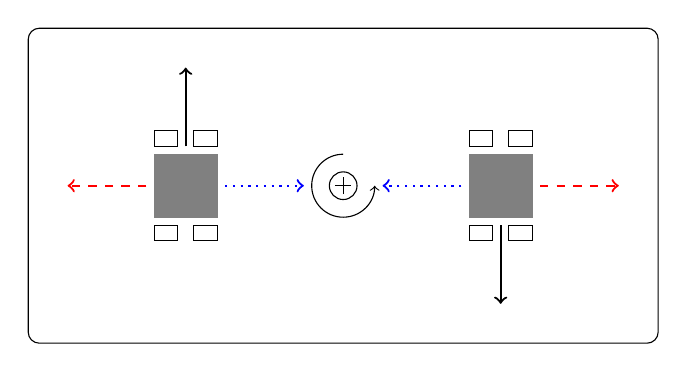
\begin{tikzpicture}
\draw[thin,rounded corners] (-4,-2) -- (4,-2) -- (4,2) -- (-4,2) -- cycle;
\draw[fill,gray] (-24mm,-4mm) rectangle +(8mm,8mm);
\draw[->,thick,dotted,blue] (-15mm,0mm) -- (-5mm,0mm);
\draw[->,thick,dashed,red] (-25mm,0mm) -- (-35mm,0mm);
\draw[->,thick] (-2,5mm) -- (-2,15mm);
\draw[fill,gray] (16mm,-4mm) rectangle +(8mm,8mm);
\draw[->,thick,dotted,blue] (15mm,0mm) -- (5mm,0mm);
\draw[->,thick,dashed,red] (25mm,0mm) -- (35mm,0mm);
\draw[->,thick] (2,-5mm) -- (2,-15mm);
\draw (0,0) circle[radius=5pt];
\draw (-3pt,0) -- (3pt,0);
\draw (0,-3pt) -- (0,3pt);
\draw[<-] (4mm,0) arc [start angle=0, end angle=-270, radius=4mm];
\foreach \x/\y in {-24/5,-19/5,16/5,21/5,-24/-7,-19/-7,16/-7,21/-7} {
  \draw (\x mm, \y mm) rectangle +(3mm,2mm);
}
\end{tikzpicture}
\end{center}
\caption{Physique d'un gyroscope à diapason : les flèches en pointillés rouges et les flèches en pointillés bleus indiquent la direction de la vibration ; les flèches noires pleines indiquent la direction de la force de Coriolis}\label{fig.tuning-gyro}
\end{figure}

\subsection{Applications}

Un système de navigation inertiel possède trois accéléromètres et trois gyroscopes afin de pouvoir calculer la position du véhicule en trois dimensions. Ceci est nécessaire pour les avions et autres véhicules robotisés. Les airbags utilisent un accéléromètre qui détecte la décélération rapide dans le sens avant-arrière qui se produit lors d'un accident de voiture. Cela provoque une expansion explosive de l'airbag. On peut imaginer d'autres applications pour ces composants dans les voitures. Un accéléromètre dans le sens haut-bas peut détecter si la voiture est tombée dans un nid-de-poule. Un gyroscope mesurant la rotation autour de l'axe vertical peut détecter un dérapage, tandis que le gyroscope mesurant la rotation autour de l'axe avant-arrière peut détecter si la voiture se retourne.


\section{Degrés de liberté et nombre d'actionneurs}\label{s.dof}
\index{degré de liberté}
\index{actionneur}

Le nombre de \emph{degrés de liberté (DOF)} d'un système est la dimensionnalité des coordonnées nécessaires pour décrire la pose d'un robot mobile ou la pose de l'effecteur final d'un manipulateur robotique.\footnote{Cette section et les suivantes sont plus avancées et peuvent être passées lors de votre première lecture. De plus, certains des exemples concernent des manipulateurs robotiques décrits dans le Chap.~\ref{ch.kinematics}.} Par exemple, un hélicoptère possède six DOF car il peut se déplacer dans les trois dimensions spatiales et tourner autour des trois axes. Par conséquent, une coordonnée à six dimensions $(x,y,z,\phi,\psi,\theta)$ est nécessaire pour décrire sa pose.

\begin{quote}
\begin{center}
\textbf{Les termes utilisés pour décrire les rotations}
\end{center}
Un hélicoptère peut tourner autour de ses trois axes. Les rotations sont appelées : (a) tangage : le nez se déplace de haut en bas ; (b) roulis : le corps tourne autour de son axe longitudinal ; (c) lacet : le corps tourne de gauche à droite autour de l'axe de son rotor.
\end{quote}

Le bras robotique à deux articulations de la Fig.~\ref{fig.two-link} ne possède que deux DOF car son effecteur final se déplace dans un plan et ne tourne pas ; il peut donc être décrit par des coordonnées bidimensionnelles $(x,y)$. En examinant à nouveau la Fig.~\ref{fig.pos-head}, vous pouvez voir qu'un robot mobile se déplaçant sur une surface plane possède trois DOF, car sa pose est définie par une coordonnée tridimensionnelle $(x,y,\theta)$. Un train n'a qu'une seule DOF car il est contraint par les rails à se déplacer en avant (ou occasionnellement en arrière) le long de la voie. Il suffit d'une seule coordonnée $(x)$, la distance du train par rapport à une origine arbitraire de la voie, pour spécifier la pose du train.


\begin{figure}
\begin{center}
% Forward kinematics
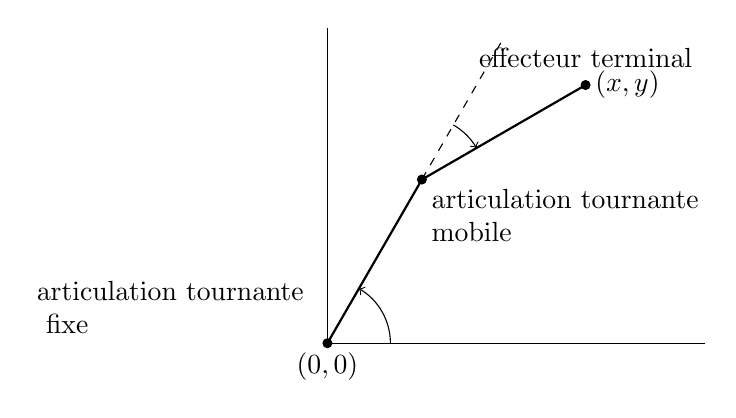
\begin{tikzpicture}[scale=.8,align=left]
\draw (0,0) coordinate (origin) -- (6,0);
\draw (origin) -- (0,5);
\draw[thick] (origin) -- ++(60:3) coordinate (prime) -- ++(30:3) coordinate (point);
\path (origin) -- ++(60:3) -- ++(30:1) coordinate (angle);
\draw[dashed] (60:3) -- ++(60:2.6);
\draw[->] (1,0) arc (0:60:1);
\draw[<-] (angle) arc (30:60:1);
\draw[fill] (origin) circle [radius=2pt] node[below] {$(0,0)$};
\draw[fill] (prime) circle [radius=2pt];
\draw[fill] (point) circle [radius=2pt] node[right] {$(x,y)$};
\node[above,yshift=1mm] at (point) {\p{effecteur terminal}};
\node[above left,xshift=-5pt] at (origin) {\p{articulation tournante}\\\p{ fixe}};
\node[below right] at (prime) {\p{articulation tournante}\\\p{mobile}};
\end{tikzpicture}
\end{center}
\caption{Un bras robotique à deux articulations avec deux DOF}\label{fig.two-link}
\end{figure}

Nous avons besoin de plus d'informations que les degrés de liberté pour décrire un mouvement robotique. Considérons un véhicule tel qu'une voiture, un vélo ou une chaise de bureau. Bien que trois coordonnées $(x,y,\theta)$ soient nécessaires pour décrire sa pose, nous ne pouvons pas nécessairement déplacer le véhicule directement d'une pose à une autre. Une chaise de bureau peut être déplacée \emph{directement} en tout point du plan et orientée dans n'importe quelle direction. Une voiture ou une bicyclette située à $(2,0,0^\circ)$ (pointée le long de l'axe positif $x$) ne peut pas être déplacée directement le long de l'axe $y$ vers la position $(2,2,0^\circ)$. Une manœuvre plus complexe est nécessaire.

Nous devons connaître le nombre de ses \emph{actuateurs} (généralement des moteurs) et leur configuration. Un robot à entraînement différentiel possède deux actionneurs, un pour chaque roue, bien que le robot lui-même ait trois DOF. Les moteurs déplacent le robot le long d'un axe en avant et en arrière, mais en appliquant une puissance inégale, nous pouvons modifier le cap du robot. Le bras à deux articulations de la Fig.~\ref{fig.two-link} possède deux moteurs, un pour chaque articulation tournante, de sorte que le nombre d'actionneurs est égal au nombre de DOF. Enfin, un train n'a qu'un seul actionneur, le moteur qui le fait avancer ou reculer dans son unique DOF.

\begin{framed}
\act{Robot qui peut seulement tourner}{rotation seulement}
\begin{itemize}
\item La figure~\ref{fig.rot-dof} montre un robot à entraînement différentiel dont le centre de rotation est traversé par une tige fixe. La tige empêche le robot de changer de position, lui permettant uniquement de tourner autour de son axe vertical. Caractérisez cette configuration : le nombre d'actionneurs et le nombre de DOF.
\item Quels types de tâches ce robot pourrait-il effectuer ? Quels sont les avantages et les inconvénients de cette configuration ?
\end{itemize}
\end{framed}

\begin{figure}
\begin{center}
\begin{tikzpicture}[scale=1.3]
\begin{scope}[rotate=30]
\coordinate (origin) at (0,0);
\pic[scale=1.6,rotate=30] at (origin) {robot};
\fill[gray!80] (origin) circle [radius=2mm];
\draw[raxis] (0,0) -- (-8pt,0);
\draw[raxis] (0,0) -- (8pt,0);
\draw[->,thick] ($(origin)+(-5pt,10pt)$) arc (130:-10:9pt);
\end{scope}
\draw[raxis] (0,0) -- (120:15mm);
\draw[raxis] (0,0) -- (300:15mm);
\end{tikzpicture}
\end{center}
\caption{Un robot qui ne peut tourner qu'autour d'un axe (point gris)}\label{fig.rot-dof}
\end{figure}

\section{Le nombre relatif d'actionneurs et de DOF}\label{s.num-actuators}

Analysons les systèmes où :
\begin{itemize}
\item Le nombre d'actionneurs est égal au nombre de DOF ;
\item Le nombre d'actionneurs est inférieur au nombre de DOF ;
\item Le nombre d'actionneurs est supérieur au nombre de DOF.
\end{itemize}

\subsection*{Le nombre d'actionneurs est égal au nombre de DOF}

Un train possède un actionneur (son moteur) qui déplace le train le long de son unique DOF. Le bras robotique à deux lignes de la Fig.~\ref{fig.two-link} possède deux actionneurs et deux DOF. Une pince robotique peut être construite avec trois moteurs qui font tourner la pince dans chacune des trois orientations (roulis, tangage, lacet). L'avantage d'avoir un nombre égal d'actionneurs et de DOF est que le système est relativement facile à contrôler : chaque actionneur est commandé individuellement pour déplacer le robot vers la position souhaitée dans le DOF qu'il contrôle.

\subsubsection*{Le nombre d'actionneurs est inférieur au nombre de DOF}

Les robots mobiles ont généralement moins d'actionneurs que de DOF. Un robot à entraînement différentiel et une voiture n'ont que deux actionneurs, mais ils peuvent atteindre toutes les positions tridimensionnelles possibles dans le plan. Le fait d'avoir moins d'actionneurs rend le système moins coûteux, mais les problèmes de planification et de contrôle du mouvement sont beaucoup plus difficiles. Le stationnement parallèle d'une voiture est réputé pour sa difficulté : deux rotations et une translation sont nécessaires pour effectuer un simple déplacement latéral (Figures~\ref{fig.parallel-diff}--\ref{fig.parallel-car}).

Un exemple extrême est celui d'une montgolfière qui ne possède qu'un seul actionneur (un réchauffeur) qui injecte plus ou moins d'air chaud dans le ballon et contrôle ainsi son altitude. Cependant, les vents peuvent faire bouger la montgolfière dans l'une des trois directions de l'espace et même la faire tourner (au moins partiellement) dans trois orientations, de sorte que l'opérateur de la montgolfière ne peut jamais la contrôler précisément. Une montgolfière diffère donc d'un ascenseur : les deux ont un seul actionneur, mais l'ascenseur est contraint par son arbre à se déplacer dans une seule DOF.

Pour un autre exemple de la relation complexe entre les DOF et le nombre d'actionneurs, le lecteur est invité à étudier la commande de vol des hélicoptères. Les hélicoptères sont très maniables (encore plus que les avions, qui ne peuvent pas voler en arrière), mais un pilote contrôle le vol de l'hélicoptère en utilisant seulement trois actionneurs :
\begin{itemize}
\item La \emph{commande de pas cyclique} contrôle le pas du \emph{arbre} du rotor principal qui détermine si l'hélicoptère se déplace en avant, en arrière ou sur un côté.
\item Le paramètre \emph{collective} contrôle le pas des \emph{pales} du rotor principal qui détermine si l'hélicoptère se déplace vers le haut ou vers le bas.
\item Les \emph{pédales} contrôlent la vitesse du rotor de queue qui détermine la direction dans laquelle le nez de l'hélicoptère pointe.
\end{itemize}

\subsubsection*{Le nombre d'actionneurs est supérieur au nombre de DOF}

Cela ne semble pas être une bonne idée d'avoir \emph{plus} d'actionneurs que de DOF, mais en pratique, de telles configurations sont souvent utiles. Les systèmes des figures~\ref{fig.hi-act-low-dof-1}--\ref{fig.hi-act-low-dof-2} ont plus d'actionneurs que de DOF. Le bras manipulateur robotique de la Fig.~\ref{fig.hi-act-low-dof-1} possède quatre liaisons tournant dans le plan avec des actionneurs (moteurs) \p{a1}, \p{a2}, \p{a3}, \p{a4} aux articulations. Nous supposons que l'effecteur final est fixé au lien de \p{a4} et ne peut pas tourner, donc sa pose est définie par sa position $(x,y)$ et une orientation fixe. Par conséquent, bien que le bras ait quatre actionneurs, il n'a que deux DOF car il ne peut déplacer l'effecteur final qu'horizontalement et verticalement.

Le robot mobile avec un bras (Fig.~\ref{fig.hi-act-low-dof-2}) possède trois actionneurs : un moteur qui déplace le robot en avant et en arrière, et des moteurs pour chacune des deux articulations tournantes. Cependant, le système n'a que deux DOF puisque la pose de son effecteur final est définie par une coordonnée bidimensionnelle $(x,y)$. Les systèmes comportant plus d'actionneurs que de DOF sont appelés \emph{systèmes redondants}\index{systèmes redondants}.

\begin{figure}
\begin{minipage}{.45\textwidth}
\begin{tikzpicture}[scale=1.2]
\coordinate (j1) at (1,0);
\fill[gray!50] (0,-2mm) rectangle +(4,-2mm);
\draw[very thick] (j1) -- +(0,-2mm);
\draw[thick] (j1) node[above right,xshift=5pt] {\p{a1}} -- ++(120:10mm) coordinate (j2) node[left,xshift=-2pt,yshift=-2pt] {\p{a2}} -- ++(30:15mm) coordinate (j3) node[above left,xshift=-4pt,yshift=-2pt] {\p{a3}} -- ++(10:12mm) coordinate (j4) node[right,xshift=2pt,yshift=-2pt] {\p{a4}} -- ++(80:8mm) coordinate (ee) node[left,xshift=-2pt] {\p{effecteur terminal}};
\draw[->] ($(j1)+(-7pt,2pt)$) arc (180:0:6pt);
\draw[->] ($(j2)+(-5pt,4pt)$) arc (140:-40:6pt);
\draw[->] ($(j3)+(-5pt,2pt)$) arc (160:-60:6pt);
\draw[->] ($(j4)+(-6pt,2pt)$) arc (180:0:6pt);
\fill (j1) circle [radius=2pt];
\fill (j2) circle [radius=2pt];
\fill (j3) circle [radius=2pt];
\fill (j4) circle [radius=2pt];
\fill (ee) circle [radius=2pt];
\end{tikzpicture}
\caption{Bras de robot : deux DOF et quatre actionneurs}\label{fig.hi-act-low-dof-1}
\end{minipage}
\hspace{\fill}
\begin{minipage}{.45\textwidth}
\begin{tikzpicture}[scale=1.2]
\fill[gray!50] (0,-3mm) rectangle +(4,-2mm);
\draw[rounded corners] (4mm,0) rectangle +(3,1);
\draw[fill=white] (11mm,0) circle [radius=3mm];
\draw[fill=white] (29mm,0) circle [radius=3mm];
\draw[raxis] (11mm,0) -- +(-2mm,0);
\draw[raxis] (11mm,0) -- +(2mm,0);
\draw[raxis] (11mm,0) -- +(0,2mm);
\draw[raxis] (11mm,0) -- +(0,-2mm);
\draw[raxis] (29mm,0) -- +(-2mm,0);
\draw[raxis] (29mm,0) -- +(2mm,0);
\draw[raxis] (29mm,0) -- +(0,2mm);
\draw[raxis] (29mm,0) -- +(0,-2mm);
\draw (17mm,1) coordinate (j1) node[above right] {\p{a1}} -- ++(130:10mm) coordinate (j2) node[left,xshift=-2pt] {\p{a2}} -- ++(60:10mm) coordinate (ee) node[right,xshift=2pt] {\p{effecteur terminal}};
\draw[->] ($(j1)+(0pt,-5pt)$) arc (-90:-270:6pt);
\draw[->] ($(j2)+(-3pt,6pt)$) arc (120:-100:6pt);
\fill (j1) circle [radius=2pt];
\fill (j2) circle [radius=2pt];
\fill (ee) circle [radius=2pt];
\end{tikzpicture}
\caption{Robot mobile et bras : deux DOF et trois actionneurs}\label{fig.hi-act-low-dof-2}
\end{minipage}
\end{figure}

Dans la mesure du possible, les ingénieurs évitent d'utiliser plus d'un actionneur agissant sur le même DOF car cela augmente la complexité et le coût d'un système. La cinématique inverse (Sect.~\ref{s.inverse-kinematics}) d'un système redondant donne lieu à un nombre infini de solutions qui compliquent le fonctionnement du système. Pour le robot mobile avec le bras (Fig.~\ref{fig.hi-act-low-dof-2}), il existe un nombre infini de positions de la base et du bras qui amènent l'effecteur final à une position atteignable spécifique.

Dans certaines situations, un système redondant est nécessaire car la tâche ne pourrait pas être exécutée avec moins d'actionneurs. La figure~\ref{fig.redundant1} montre comment le bras robotique à quatre liaisons de la figure~\ref{fig.hi-act-low-dof-1} peut déplacer l'effecteur final vers une position qui est bloquée par un obstacle et donc inaccessible par un bras à deux liaisons (figure~\ref{fig.redundant2}), même si dans les deux configurations la longueur totale des liaisons est égale.

\begin{figure}
\begin{minipage}{.45\textwidth}
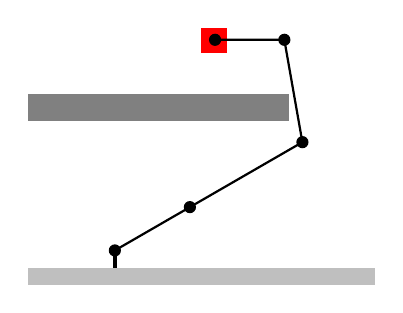
\begin{tikzpicture}[scale=1.1]
\coordinate (j1) at (1,0);
\fill[gray!50] (0,-2mm) rectangle +(4,-2mm);
\draw[very thick] (j1) -- +(0,-2mm);
\draw[fill,gray] (0,15mm) rectangle +(30mm,3mm);
\draw[red,fill] (57pt,65pt) rectangle +(8pt,8pt);
%\draw (0,0) -- (1,0) coordinate (j1)-- (4,0);
\draw[thick] (j1) -- ++(30:10mm) coordinate (j2) -- ++(30:15mm) coordinate (j3) -- ++(100:12mm) coordinate (j4) -- ++(180:8mm) coordinate (ee);
\fill (j1) circle [radius=2pt];
\fill (j2) circle [radius=2pt];
\fill (j3) circle [radius=2pt];
\fill (j4) circle [radius=2pt];
\fill (ee) circle [radius=2pt];
\end{tikzpicture}
\caption{Arm with four actuators can reach a hidden position}\label{fig.redundant1}
\end{minipage}
\hspace{\fill}
\begin{minipage}{.45\textwidth}
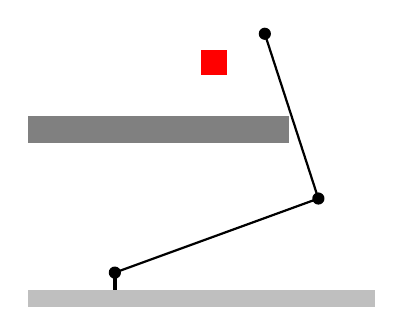
\begin{tikzpicture}[scale=1.1]
\coordinate (j1) at (1,0);
\fill[gray!50] (0,-2mm) rectangle +(4,-2mm);
\draw[very thick] (j1) -- +(0,-2mm);
\draw[fill,gray] (0,15mm) rectangle +(30mm,3mm);
\draw[red,fill] (57pt,65pt) rectangle +(8pt,8pt);
%\draw (0,0) -- (1,0) coordinate (j1)-- (4,0);
\draw[thick] (j1) -- ++(20:25mm) coordinate (j2) -- ++(108:20mm) coordinate (ee);
\fill (j1) circle [radius=2pt];
\fill (j2) circle [radius=2pt];
\fill (ee) circle [radius=2pt];
\end{tikzpicture}
\caption{Arm with two actuators is blocked by an obstacle}\label{fig.redundant2}
\end{minipage}
\end{figure}

Un avantage important des systèmes redondants provient des actionneurs ayant des caractéristiques différentes. Le robot mobile de la Fig.~\ref{fig.hi-act-low-dof-2} peut s'approcher rapidement de la cible, bien que sa position finale puisse ne pas être précise en raison d'erreurs comme un terrain accidenté. Une fois que le robot mobile s'arrête, les moteurs des articulations qui n'ont pas à faire face au terrain peuvent être positionnés avec précision. Bien que le positionnement soit précis, ces articulations n'ont pas la portée étendue de la base mobile.

\subsection*{Exemple d'un système comportant plus d'actionneurs que de DOF}

La figure~\ref{fig.act-dof} (vues de dessus et de côté) montre une configuration avec \emph{deux actionneurs et une DOF}. Le système modélise une grue robotisée qui déplace un poids lourd vers une position verticale spécifique. La figure~\ref{fig.crane} montre une grue construite à partir d'un robot Thymio et de composants \lego{}.\footnote{Le treuil est à droite du robot et non à gauche comme dans la figure~\ref{fig.act-dof}.}

\begin{figure}
\begin{center}
\begin{tikzpicture}[align=left]
%
% Top view
%
\begin{scope}[scale=2,xshift=25mm]
% Table
\draw[fill,gray!20] (-34mm,-26mm) rectangle +(40mm,30mm);
% Robot
\draw (0,0) to [rounded corners] (-20mm,0) to [rounded corners, bend right=45] (-20mm,-18mm) to (0,-18mm) to cycle;
% Drive wheels
\fill (-11mm,0) rectangle +(8mm, 2mm);
\fill (-11mm,-18mm) rectangle +(8mm, -2mm);
\node at (-12mm,-8mm) {\p{roues motrices}};
\draw[->] (-8mm,-6mm) -- +(0,14pt);
\draw[->] (-8mm,-10mm) -- +(0,-20pt);
% Road wheels
\fill[gray!70] (-3mm,0) rectangle +(10mm, 2mm) node[above left,black,xshift=-38pt,yshift=13pt] {\p{roue de route}};
\draw[->] (1mm,5mm) -- +(0,-8pt);
\fill[gray!70] (-3mm,-23mm) rectangle +(10mm, -2mm);
\draw[fill,cyan] (2mm,0) rectangle +(2pt,-23mm);
\draw[fill,cyan] (2mm,-9mm) rectangle +(-4mm,2pt);
\draw[raxis] (2.4mm,-25.6mm) -- +(0,29mm);
% Winch
\fill[red] (-9mm,-20mm) rectangle +(4mm, -2mm) node[below left,black,xshift=-18pt,yshift=-7pt] {\p{treuil}};
\draw[->] (-8mm,-25mm) -- +(0,8pt);
\draw[raxis] (-7mm,-24mm) -- +(0,27mm);
% Weight
\fill[red] (-41.1mm,-22mm) rectangle +(1.5mm,2mm);
% Bearing
\fill[gray!70] (-40mm,-22.8mm) rectangle +(2mm,4mm) node[above,xshift=-4mm,black,yshift=6pt] {\p{palier et}\\\p{poids}};
\draw[raxis] (-39mm,-23.8mm) -- +(0,6mm);
% Cable
\draw[thick,red] (-9mm,-21mm) -- ++(-32mm,0);
\end{scope}
%
% Side view
%
\begin{scope}[scale=.8,yshift=-10.5cm]
% Table
\draw[fill,gray!20] (-2,-23.5mm) rectangle +(9.5,2mm);
\draw[fill,gray!20] (-1,-23.5mm) rectangle +(4mm,-15mm);
\draw[fill,gray!20] (5,-23.5mm) rectangle +(4mm,-15mm);
% Big wheel
\draw[fill,gray!70] (62mm,-9mm) circle[radius=1.25] node[left,black,xshift=-34pt,yshift=-8pt] {\p{roue de route}};
% Attachment
\draw[fill,cyan] (62mm,-9mm) circle[radius=4pt];
\draw[fill,cyan] (61.5mm,-9mm) rectangle +(3pt,20.5mm);
\draw[fill,cyan] (62.5mm,11mm) rectangle +(-5mm,3pt);
% Axis intersection of big wheel
\draw[raxis] (62mm,-9mm) -- +(24pt,0);
\draw[raxis] (62mm,-9mm) -- +(-24pt,0);
\draw[raxis] (62mm,-9mm) -- +(0,24pt);
\draw[raxis] (62mm,-9mm) -- +(0,-24pt);
% Robot
\draw[rounded corners,fill=white] (.2,0) -- (.2,2) -- (5.9, 2) -- (5.9,0) -- cycle;
% Wheel
\draw[fill,black] (4.3,9pt) circle[radius=1] node[left,black,xshift=-24pt,yshift=23pt] {\p{roues motrices}};
% Winch
\draw[fill,red]  (4.3,9pt) circle[radius=.5] node[above right,black,xshift=5pt,yshift=28pt] {\p{treuil}};
\draw[->] (5,39pt) -- +(-16pt,-24pt);
\draw[raxis] (4.3,9pt) -- +(14pt,0);
\draw[raxis] (4.3,9pt) -- +(-14pt,0);
\draw[raxis] (4.3,9pt) -- +(0,14pt);
\draw[raxis] (4.3,9pt) -- +(0,-14pt);
% Support
\draw[fill,gray!70] (.9,0) rectangle +(.8,-17.5mm);
\draw[fill,gray!70] (.9,-17.5mm) arc(180:360:4mm);
% Bearing
\draw[red,fill=gray!70] (-85pt,13pt) circle[radius=10pt] node[above,black,yshift=4mm] {\p{bearing}};
\draw[thick,red] (4.3,23pt) -- (-85pt,23pt);
\draw[raxis] (-85pt,13pt) -- +(8pt,0);
\draw[raxis] (-85pt,13pt) -- +(-8pt,0);
\draw[raxis] (-85pt,13pt) -- +(0,8pt);
\draw[raxis] (-85pt,13pt) -- +(0,-8pt);
% Weight
\draw[thick,red] (-95pt,13pt) -- ++(0,-100pt);
\draw[fill,red] (-101pt,-95pt) rectangle +(12pt,12pt) node[right,black] {\p{poids}};
\end{scope}
\end{tikzpicture}
\caption{Grue robotique construite à partir d'un robot mobile et d'un treuil (vue de dessus en haut, vue de côté en bas) ; sur la vue de côté, la roue gauche n'est pas représentée}\label{fig.act-dof}
\end{center}
\end{figure}

\begin{figure}
\begin{center}
\includegraphics[width=.8\textwidth]{robotic-crane.jpg}
\caption{Grue robotique construite à partir d'un robot Thymio et de composants \lego{}}\label{fig.crane}
\end{center}
\end{figure}

Le système est construit à partir d'un robot mobile à entraînement différentiel, mais les roues ne sont pas directement utilisées pour contrôler le mouvement du système. Au lieu de cela, chaque roue est un actionneur indépendant. (Rappelez-vous que la puissance de chaque roue d'un robot à entraînement différentiel peut être réglée indépendamment sur n'importe quelle valeur dans une plage telle que $-100$ à $100$).

Le robot est orienté vers la gauche. La roue motrice droite de la Fig.~\ref{fig.act-dof} (le rectangle noir en haut de la vue de dessus et caché derrière le robot dans la vue de côté) commande une paire de roues de route (grises) qui déplacent rapidement le robot en avant et en arrière. À son tour, le câble fait monter et descendre rapidement le poids.

Les roues sont montées sur une structure (en bleu) qui est fixée au corps du robot. Il existe plusieurs options pour transférer la puissance de la roue motrice droite aux roues de la route : friction, poulies et courroies, et engrenages. Chaque option a ses propres avantages et inconvénients, et les trois sont utilisées dans les voitures : l'embrayage utilise la friction, les courroies sont utilisées pour la synchronisation et pour faire fonctionner les composants auxiliaires comme les pompes à eau, et les engrenages sont utilisés dans la transmission pour contrôler le couple appliqué à chaque roue.

La roue motrice gauche (le rectangle noir en bas de la vue de dessus et à l'avant de la vue latérale) commande un treuil (rouge) qui enroule ou déroule un câble attaché au poids qui monte ou descend sur un roulement fixe. Le diamètre du treuil est beaucoup plus petit que celui des roues motrices, de sorte qu'il peut déplacer le poids par petits incréments lorsque la roue motrice gauche tourne. L'objectif de la conception est de pouvoir effectuer un positionnement précis du poids même si le treuil déplace le câble à une vitesse beaucoup plus lente que le corps du robot.

Deux activités sont prévues dans cette section. La première activité s'adresse aux lecteurs qui possèdent de bonnes compétences en construction et un kit robotique approprié. La seconde activité propose d'autres moyens de démontrer le concept de deux actionneurs dans un DOF.

\begin{framed}
\act{Grue robotique}{act-dof}
\begin{itemize}
\item Construisez la grue robotisée représentée sur la Fig.~\ref{fig.act-dof}. Expliquez votre choix de mécanisme pour relier la roue motrice aux roues de la route.
\item Écrivez un programme qui, étant donné la position actuelle du poids et une position cible, déplace le poids vers la position cible. Vous pouvez également envoyer des commandes aux moteurs à l'aide d'une télécommande ou d'un ordinateur connecté au robot.
\item Expérimentez les vitesses de rotation relatives des roues motrices gauche et droite qui contrôlent respectivement les roues de la route et le treuil. Devez-vous déplacer les deux actionneurs séparément ou simultanément ?
\end{itemize}
\end{framed}

\begin{framed}
\act{Grue robotique (alternatives)}{act-dof-alt}
\begin{itemize}
\item Écrivez un programme qui permet à un robot mobile de se déplacer en avant et en arrière. Placez un morceau de ruban adhésif noir relativement loin de la position initiale du robot. L'objectif est de faire en sorte que le robot s'arrête le plus près possible du début du ruban, sans vérifier continuellement le capteur. 
\item Le programme comporte trois modes de fonctionnement. (1) Le robot se déplace rapidement, vérifie occasionnellement son capteur et s'arrête lorsqu'il détecte la bande. (2) Comme en (1), mais le robot se déplace lentement, en vérifiant son capteur relativement souvent. (3) Comme en (1) mais lorsque la bande est détectée, le robot recule en utilisant la vitesse et la période d'échantillonnage comme en (2).
\item Exécutez le programme et comparez les résultats des trois modes : le temps jusqu'à l'arrêt du robot et l'erreur entre la position finale du robot et le début de la bande.
\item Vous pouvez également exécuter le programme avec les trois modes sur un ordinateur et expérimenter les paramètres de mouvement et les périodes d'échantillonnage. Vous devrez choisir un modèle pour le mouvement : vitesse constante, accélération constante ou (de façon plus réaliste) accélération puis vitesse constante et enfin décélération lorsque la bande est détectée.
\end{itemize}
\end{framed}

\section{Mouvement holonome et non holonome}\label{s.holonomic}

La section~\ref{s.dof} a présenté le concept de degré de liberté (DOF) et le rôle du nombre d'actionneurs. Il existe un autre concept qui relie les DOF et les actionneurs dans le cas d'un robot mobile : le \emph{degré de mobilité (DOM)}\index{degré de mobilité}. Le degré de mobilité $\delta_m$ correspond au nombre de degrés de liberté auxquels les actionneurs peuvent \emph{directement accéder}. Un robot mobile dans le plan possède au maximum trois DOF (position et cap $(x,y)$), le degré maximal de mobilité d'un robot mobile est donc $\delta_m = 3$.

Considérons les DOM de différents véhicules. Un train n'a qu'un seul degré de liberté parce qu'il ne peut que se déplacer vers l'avant le long des rails, et il a un seul actionneur, son moteur, qui affecte directement cet unique degré de liberté. Par conséquent, un train a un degré de mobilité de $\delta_m = 1$, ce qui signifie que l'actionneur peut accéder directement à l'unique DOF.

Un robot à entraînement différentiel possède trois DOF. Les deux actionneurs sont les deux moteurs qui agissent sur les roues. Ils peuvent accéder directement à deux DOF : (a) si les deux roues tournent à la même vitesse, le robot avance ou recule ; (b) si les roues ont des vitesses opposées, le robot tourne sur place. Par conséquent, nous pouvons accéder directement aux DOF le long de l'axe de translation avant et aux DOF du cap, mais nous ne pouvons pas accéder directement aux DOF de l'axe de translation latéral (Fig.~\ref{fig.mobility-example1}). Un robot mobile à entraînement différentiel a un degré de mobilité $\delta_m = 2 < 3 = \#\textrm{DOF}$.

\begin{figure}
\begin{minipage}{.45\textwidth}
\begin{tikzpicture}[align=left,scale=.9]
\coordinate (origin) at (0,0);
\pic[scale=2.2] at (origin) {robot};
\draw[<-,thick] ($(origin)+(4pt,20pt)$) arc (90:-90:20pt);
\draw[->,thick] ($(origin)+(10pt,0)$) -- +(95pt,0);
\node at (18mm,-9mm) {\p{accessible}\\\p{DOF}};
\draw[->] (18mm,-5mm) -- +(0,4mm);
\draw[->] (15mm,-5mm) -- +(-5mm,2mm);
\draw[->,thick,dashed] ($(origin)+(0,5pt)$) -- +(0,85pt);
\node at (18mm,26mm) {\p{non accessible}\\\p{DOF}};
\draw[->] (6mm,26mm) -- +(-5mm,0);
\end{tikzpicture}
\caption{DoF accessibles et non accessibles pour un robot avec entraînement différentiel}\label{fig.mobility-example1}
\end{minipage}
\hspace{\fill}
\begin{minipage}{.5\textwidth}
\begin{tikzpicture}[baseline=-20pt,align=left,scale=1.2]
\draw[rounded corners] (0,0) -- ++(4,0) -- ++(0,2) -- ++(-4,0) -- cycle;
\draw[rounded corners] (.5,.5) -- ++(1.5,0) -- ++(0,1) -- ++(-1.5,0) -- cycle;
\draw (.1,.1) -- (.5,.5);
\draw (.1,1.9) -- (.5,1.5);
\draw (2.4,.1) -- (2,.5);
\draw (2.4,1.9) -- (2,1.5);
\draw (2.5,.1) -- +(0,1.8);
\draw[<-,thick,dashed] (2.8,1.5) arc (90:-90:15pt);
\draw[->,thick] (3,1) -- +(45pt,0);
\draw[->,thick,dashed] (1.25,1) -- +(0,50pt);
\draw[fill,rotate around={30:(3.4,-.1)}] (3,-.2) rectangle +(.8,.2);
\draw[fill,rotate around={30:(3.4,2.1)}] (3,2) rectangle +(.8,.2);
\draw[fill] (.3,-2mm) rectangle +(.8,2mm);
\draw[fill] (.3,2) rectangle +(.8,2mm);
\node at (22mm,-4mm) {\p{accessible}\\\p{DOF}};
\draw[->] (26mm,-1mm) -- +(11mm,10mm);
\node at (26mm,25mm) {\p{non accessible}\\\p{DOF}};
\draw[->] (17mm,24mm) -- +(-4mm,0);
\draw[->] (25mm,23mm) -- +(4mm,-7mm);
\draw[raxis] (.7,-6mm) -- +(0,10mm);
\draw[raxis] (.7,16mm) -- +(0,10mm);
\draw[raxis] (3.4,-.1) -- +(120:4mm);
\draw[raxis] (3.4,-.1) -- +(300:4mm);
\draw[raxis] (3.4,2.1) -- +(120:4mm);
\draw[raxis] (3.4,2.1) -- +(300:4mm);
\end{tikzpicture}
\caption{DoF accessibles et non accessibles pour un robot avec direction Ackermann}\label{fig.mobility-example2}
\end{minipage}
\end{figure}

Une voiture, comme un robot à entraînement différentiel, ne dispose que de deux actionneurs pour trois DOF : un actionneur, le moteur, donne un accès direct au degré de liberté selon l'axe longitudinal de la voiture, ce qui lui permet d'avancer et de reculer. L'autre actionneur, le volant, ne donne pas d'accès direct à d'autres DOF, il ne peut qu'orienter le premier DOF. La voiture ne peut pas tourner autour de l'axe vertical et elle ne peut pas se déplacer latéralement (Fig.~\ref{fig.mobility-example2}). Par conséquent, une voiture n'a qu'un seul degré de mobilité, $\delta_m = 1$. Intuitivement, vous pouvez constater le degré de mobilité inférieur d'une voiture par rapport à un robot à entraînement différentiel en notant que le robot peut tourner sur place alors que la voiture ne le peut pas.

En soi, une roue standard a $\delta_m=2$ : elle peut rouler en avant et en arrière et tourner autour de l'axe vertical qui passe par le point de contact de la roue avec le sol. Une roue ne peut pas se déplacer latéralement, ce qui est en fait une bonne chose car cela empêche le véhicule de déraper sur la route dans un virage. Dans la voiture, le degré de mobilité est encore réduit à $\delta_m=1$, car il y a deux paires de roues, une à l'avant et une à l'arrière de la voiture. Cette configuration rend impossible la rotation de la voiture autour de son axe vertical, même si les roues individuelles peuvent le faire (généralement uniquement les roues avant). La limitation à $\delta_m=1$ donne de la stabilité à la voiture - elle ne peut pas déraper latéralement et elle ne peut pas tourner - ce qui rend la conduite à grande vitesse facile et sûre. En fait, un accident peut se produire lorsque la pluie ou la neige réduit la friction de sorte que la voiture peut déraper ou tourner.

Un robot mobile autonome peut en profiter s'il a un DOM supérieur $\delta_m = 3$. Pour accéder directement à la troisième DOF, le robot doit être capable de se déplacer latéralement. Une méthode consiste à faire rouler le robot sur une boule ou une roue pivotante comme une chaise de bureau. Une autre méthode consiste à utiliser des \emph{roues suédoises}\index{roues suédoises} (Fig.~\ref{fig.swheel}). Une roue suédoise est une roue standard qui possède de petites roues libres le long de sa jante afin qu'elle puisse se déplacer latéralement, ce qui permet un accès direct à la troisième DOF.

\begin{figure}
\begin{minipage}{.45\textwidth}
\includegraphics[width=0.45\textwidth]{omni-dir-wheel.jpg}
\caption{Swedish wheel}\label{fig.swheel}
\end{minipage}
\hspace{\fill}
\begin{minipage}{.45\textwidth}\includegraphics[width=0.5\textwidth]{omnirobot.jpg}
\caption{Omnidirectional robot (Courtesy LAMI-EPFL)}\label{fig.omni-robot}
\end{minipage}
\end{figure}

Les robots mobiles qui peuvent accéder directement aux trois DOF ($\delta_m=3$) sont appelés \emph{robots omnidirectionnels}\label{robot omnidirectionnel}. La figure~\ref{fig.omni-robot} montre un robot omnidirectionnel construit avec quatre roues suédoises. Les deux paires de roues situées sur les côtés opposés du robot peuvent directement déplacer le robot à gauche, à droite, en avant et en arrière. Cette configuration est redondante mais très facile à contrôler. Pour éviter la redondance, la plupart des robots omnidirectionnels ont trois roues suédoises montées à un angle de $120^\circ$ les unes des autres (Figh.~\ref{fig.omni3}). Cette configuration a $\delta_m=3$ mais n'est pas facile à contrôler en utilisant les coordonnées familières $x,y$.

\begin{figure}
\begin{center}
\begin{tikzpicture}[scale=0.8]
% Draw body of robot
\draw[fill,gray!20] (0,0) circle [radius=50pt];
% Draw three Swedish wheels
\foreach \r/\x/\y in {0/0/0,120/0cm/0cm,-120/0cm/0cm} {
	\begin{scope}[xshift=\x,yshift=\y,rotate=\r]
		% Draw axle
		\draw[thick,fill,gray] (-3,-0.1) rectangle +(-.5,.2);
		% Draw motor
		\draw[thick] (-3,-.5) rectangle +(2,1);
		% Draw wheel
		\draw[rounded corners,thick,fill=gray!20] (-4,-1) to [bend right=10] ++(.5,0)
		       -- ++(0,2) to [bend right=10] ++(-.5,0) -- cycle;
		\foreach \i in {-.8,-.2,.4} {
		  \draw[rounded corners,fill=gray] (-3.85,\i) rectangle +(.2,.4);
	  }
	\end{scope}
}
% Draw axes
\foreach \r/\x/\y/\len in {60/0/0/4.5cm,180/0cm/0cm/6cm,-60/0cm/0cm/4.5cm} {
	\begin{scope}[xshift=\x,yshift=\y]
	  \draw[raxis] (0,0) -- +(\r:\len);
  \end{scope}
}
\draw[->] (-3.75,1) -- +(0,.5) node[right] {\p{mouvement entraîné}};
\draw[->,thick] (-4,0) -- +(-1,0) node[above,xshift=-2mm] {\p{mouvement libre}};
\node[xshift=-1.6cm,yshift=.2cm] at (0,0) {\p{moteur}};
\end{tikzpicture}
\end{center}
\caption{Robot omnidirectionnel avec trois roues suédoises}\label{fig.omni3}
\end{figure}

Les valeurs relatives des DOF et des DOM d'un robot définissent le concept de mouvement holonom. Un robot a un \emph{mouvement holonome} si $\delta_m = \#\textrm{DOF}$ et il a un \emph{mouvement non holonome} $\delta_m < \#\textrm{DOF}$. Un robot holonome comme celui de la figure~\ref{fig.omni-robot} peut contrôler directement toutes ses DOF sans manœuvres difficiles. La figure~\ref{fig.parallel-omni} montre à quel point il est facile pour le robot omnidirectionnel à roues suédoises (Fig.~\ref{fig.omni3}) d'effectuer un stationnement parallèle.

\begin{figure}
\begin{center}
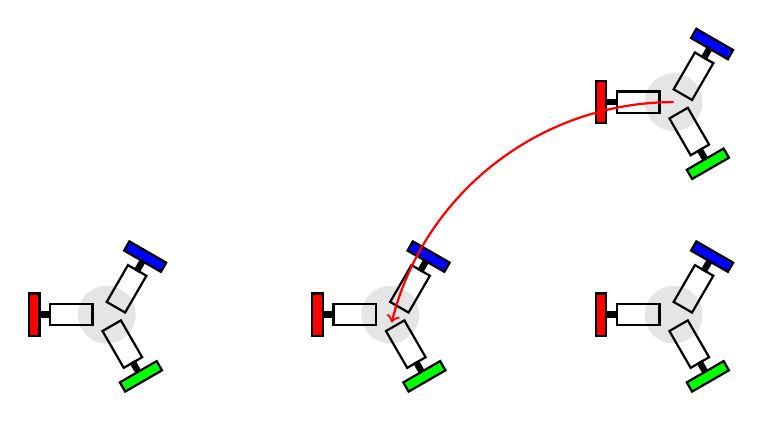
\begin{tikzpicture}[scale=.9]
\foreach \a/\b in {0/0,-40mm/-30mm,-80mm/-30mm,0/-30mm} {
	\draw[fill,gray!20] (\a,\b) circle [radius=4mm];
	\foreach \r/\x/\y/\color in
       {0/-8mm/-1.5mm/red,120/5mm/-6mm/green,-120/3mm/7mm/blue} {
		 \begin{scope}[xshift=\x+\a,yshift=\y+\b,rotate=\r,scale=.3]
			% Draw axle
			\draw[thick,fill,gray] (0,.4) rectangle +(-.5,.2);
			% Draw motor
			\draw[thick] (0,0) rectangle +(2,1);
			% Draw wheel
			\draw[thick,fill=\color] (-1,-.5) to ++(.5,0)
	       -- ++(0,2) to ++(-.5,0) -- cycle;
		 \end{scope}
	}
}
\draw[thick,red,->] (0,0) arc (90:166:41mm);
\end{tikzpicture}
\end{center}
\caption{Stationnement en parallèle par un robot omnidirectionnel}\label{fig.parallel-omni}
\end{figure}

Une voiture et un robot à entraînement différentiel sont non ergonomiques car leur DOM ($\delta_m=1$ et $\delta_m=2$, respectivement) est inférieur à leur DOF qui est de trois. En raison de ce degré de mobilité limité, ces véhicules ont besoin de manœuvres de direction complexes, par exemple pour effectuer un stationnement parallèle. Il existe une différence significative entre les deux véhicules. Le robot à entraînement différentiel nécessite trois mouvements distincts, mais ils sont très simples (Fig.~\ref{fig.parallel-diff}) : rotation à gauche, recul, rotation à droite. La voiture a également besoin de trois mouvements distincts, mais ils sont extrêmement difficiles à exécuter correctement (Fig.~\ref{fig.parallel-car}). Vous devez estimer le point de départ de la manœuvre, la précision de chaque virage et la distance à parcourir entre les virages. Le DOM supérieur du robot à entraînement différentiel est avantageux dans cette situation.

\begin{figure}
\begin{minipage}{.45\textwidth}
\begin{tikzpicture}
\pic[scale=.5] at (-14mm,-4mm) { robot };
\pic[scale=.5] at (18mm,-4mm) { robot };
\pic[scale=.5] at (2mm,15mm) { robot };
\pic[rotate=90,scale=.5] at (2mm,15mm) { robot };
\pic[scale=.5] at (2mm,-4mm) { robot };
\pic[rotate=90,scale=.5] at (2mm,-4mm) { robot };
\draw[->,thick,green!60!black] (2mm,10mm) -- +(0,-6mm);
\draw[thick,red,->] (2mm,-4mm) arc (180:90:5mm);
\draw[thick,blue,->] (2mm,15mm) arc (0:90:5mm);
\end{tikzpicture}
\caption{Parallel parking for a non-holonomic differential drive robot}\label{fig.parallel-diff}
\end{minipage}
\hspace{\fill}
\begin{minipage}{.45\textwidth}
\begin{tikzpicture}
\pic[scale=.5] at (-14mm,-4mm) { car };
\pic[scale=.5] at (18mm,-4mm) { car };
\pic[scale=.5] at (20mm,15mm) { car };
\draw[thick,red,->] (18mm,15mm) arc (90:180:10mm);
\draw[thick,blue,->] (8mm,6mm) arc (0:-90:10mm);
\draw[thick,green!60!black,->] (-1mm,-4mm) -- (12mm,-4mm);
\end{tikzpicture}
\caption{Stationnement en parallèle pour une automobile non holonome}\label{fig.parallel-car}
\end{minipage}
\end{figure}

\begin{framed}
\act{Mouvement holonome et non-holonome}{holonom}
\begin{itemize}
\item Regardez à nouveau le robot mobile qui est contraint à un mouvement de rotation uniquement (Fig.~\ref{fig.rot-dof}). Quel est son degré de mobilité $\delta_m$ ? Est-il holonome ou non ?
\item La figure~\ref{fig.wallcleaning} montre un robot qui nettoie les murs d'un bâtiment. Il y a deux ancrages d'où descendent des câbles qui passent par des yeux fixés au corps du robot, puis par des treuils actionnés par les roues du robot. En enroulant et déroulant les câbles, le robot monte et descend le long du mur. Cependant, si les deux moteurs ne font pas bouger les roues précisément à la même vitesse de rotation, le robot se balancera d'un côté à l'autre. Combien de DOF et combien de DOM ce robot possède-t-il ? Est-il holonome ou non ?
\end{itemize}
\end{framed}


\begin{figure}
\begin{center}
\begin{tikzpicture}[scale=1.2]
% Robot
\pic[rotate=90,scale=1.3] at (0,0) { robot };
% Left and right
\foreach \sign in {1,-1} {
  % Winch
  \draw (\sign*8.5mm,-1mm) rectangle +(\sign*3mm,2mm);
  \draw[fill] (\sign*11.5mm,-2mm) rectangle +(\sign*1mm,4mm);
  % Cable on winch
  \foreach \x in {9mm,9.5mm,10mm,10.5mm,11mm} {
    \draw[red] (\sign*\x,-1mm) -- +(0mm,2mm);
  }
  % Cable
  \draw[red,thick] (\sign*10mm,0mm) -- (\sign*10.8mm,18.5mm) -- (\sign*30mm,45mm);
  % Eyes
  \draw (\sign*10.8mm,18.5mm) circle [radius=.8mm];
  % Anchors
  \draw[fill,gray] (\sign*30mm,45mm) circle [radius=1mm];
}
\draw[fill,gray] (-.5mm,10mm) rectangle +(1mm,8mm); 
\draw[fill,gray] (-10mm,18mm) rectangle +(20mm,1mm);
\node at (0,45mm) {\p{ancres}};
\draw[->] (6mm,45mm) -- +(20mm,0);
\draw[->] (-6mm,45mm) -- +(-20mm,0);
\begin{scope}[yshift=5mm]
\node at (-22mm,0mm) {\p{treuil}};
\node at (22mm,0mm) {\p{treuil}};
\draw[->] (-18mm,0mm) -- +(5mm,-2mm);
\draw[->] (18mm,0mm) -- +(-5mm,-2mm);
\end{scope}
\draw[raxis] (-18mm,0mm) -- (18mm,0mm);
\end{tikzpicture}
\end{center}
\caption{Robot pour nettoyer un mur}\label{fig.wallcleaning}
\end{figure}

\section{Résumé}

Un robot mobile comme une voiture autonome ou un explorateur de Mars ne disposera pas toujours de points de repère pour sa navigation. L'odométrie est utilisée pour amener le robot à proximité de son objectif sans référence à l'environnement. Le robot estime sa vitesse et sa vélocité de rotation à partir de la puissance appliquée à ses moteurs. L'odométrie peut être améliorée en utilisant des encodeurs de roue pour mesurer le nombre de tours des roues, plutôt que de déduire la vitesse de rotation à partir de la puissance du moteur. Le changement de position d'un robot bon marché se déplaçant en ligne droite peut être calculé en multipliant la vitesse par le temps. Si le robot tourne, des calculs trigonométriques sont nécessaires pour calculer la nouvelle position et l'orientation. Même avec des encodeurs de roue, l'odométrie est sujette à des erreurs qui peuvent être très importantes si l'erreur porte sur le cap.

La navigation inertielle utilise des accéléromètres et des gyroscopes pour améliorer la précision de l'odométrie. L'intégration de l'accélération donne la vitesse et l'intégration de la vitesse angulaire donne le cap. Les systèmes micro-électromécaniques ont rendu la navigation inertielle suffisamment bon marché pour être utilisée en robotique.

Les DOF d'un système sont le nombre de dimensions dans lesquelles il peut se déplacer - jusqu'à trois dimensions sur une surface et jusqu'à six dimensions dans l'air ou sous l'eau - mais un robot peut être contraint d'avoir moins que le nombre maximum de DOF. Une autre considération est le nombre et la configuration des actionneurs d'un robot qui définissent son degré de mobilité. Si le DOM est égal au nombre de DOF, le robot est holonome et peut se déplacer directement d'une pose à une autre, bien qu'il puisse être difficile à contrôler. Si le DOM est inférieur au nombre de DOF, le robot est non ergonomique ; il ne peut pas se déplacer directement d'une pose à l'autre et devra effectuer des manœuvres complexes pour réaliser certaines tâches.

\section{Pour aller plus loin}

Un traitement mathématique détaillé des erreurs d'odométrie en deux dimensions est donné dans \cite[Sect.~5.24]{siegwart}. Pour un aperçu de la navigation inertielle, voir \cite{king,oxford}. Les manuels avancés sur la robotique présentent l'holonomie : \cite{correll,craig,siegwart,spong}.
